\documentclass[12pt]{article}
\usepackage[letterpaper,top=2cm,bottom=2cm,left=2cm,right=2cm,marginparwidth=1.75cm]{geometry}
\usepackage[utf8]{inputenc}
\usepackage{multirow}
\usepackage[utf8]{vietnam}
\usepackage{float}
\usepackage{indentfirst}
\usepackage{caption}
\usepackage{amsmath}
\usepackage{graphicx}
\usepackage[colorinlistoftodos]{todonotes}
\usepackage{listings}
\usepackage{hyperref}
\hypersetup{
    colorlinks=true,
    linkcolor=blue,
    filecolor=magenta,      
    urlcolor=cyan,
}


\begin{document}
\begin{titlepage}

    \newcommand{\HRule}{\rule{\linewidth}{0.5mm}}

    \center

    \textsc{\LARGE Đại học Khoa học tự nhiên}\\[1.5cm]
    \textsc{\Large Khoa Công nghệ thông tin}\\[0.5cm]
    \textsc{\large Môn học: Phát triển phần mềm cho thiết bị di động }\\[0.5cm]

    \HRule \\[0.4cm]
    { \huge \bfseries Báo cáo đồ án cuối kỳ\\Clover - Ứng dụng mua sắm thời trang}\\[0.4cm]
    \HRule \\[1.5cm]

    \begin{minipage}{1.\textwidth}
        \begin{flushleft} \large
            \textbf{Nhóm 9}\\
            20424008 - Dương Mạnh Cường (trưởng nhóm)\\
            19424015 - Dương Trọng Đức\\
            20424013 - Phạm Nguyễn Mỹ Diễm
        \end{flushleft}
    \end{minipage}\\[2cm]

    
\includegraphics{images/logo.png}\\[1cm]

    \today
\end{titlepage}

\section{Giới thiệu về đồ án}
\subsection{Tự đánh giá}
\textbf{10 điểm}. Nhóm bắt đầu nghiên cứu và code đồ án từ ngày 23/11/2021 và cho đến ngày 02/01/2022 thì nhóm đã hoàn thành xong đồ án. Đồ án được nhóm tìm hiểu và nghiên cứu một vài phần nằm ngoài hướng dẫn của giáo viên.

\subsection{Mô tả đồ án}
\subsubsection{Tên của đồ án}

Ứng dụng của nhóm có tên là \textbf{Clover} - một ứng dụng mua sắm thòi trang online.

\subsubsection{Môi trường thực thi}
Android Studio Arctic Fox.\\\\
\indent Ứng dụng được viết bằng ngôn ngữ Java 8.\\\\
\indent Sử dụng CSDL NoSQL Firebase Firestore do Google cung cấp.\\\\
\indent Sử dụng Firebase Firestorage của Google để lưu trữ hình ảnh.\\\\
\indent Đăng nhập người dùng qua dịch vụ Firebase Authentication.

\subsubsection{Mục tiêu của ứng dụng}
Ứng dụng được viết cho các doanh nghiệp kinh doanh trong lĩnh vực thời trang mong muốn thương hiệu của mình có một mobile application.\\\\
\indent \textbf{Về phía khách hàng}: Họ dễ dàng mua sắm, theo dõi các chương trình khuyến mãi, các sản phẩm mới ở phía nhãn hàng thời trang mà họ quan tâm.\\\\
\indent \textbf{Về phía doanh nghiệp}: Cung cấp cho doanh nghiệp một công cụ để quảng cáo cũng như kinh doanh các sản phẩm của mình, các sản phẩm được đưa đến cho khách hàng dưới góc nhìn chuyên nghiệp, tăng giá trị thương hiệu.

\subsubsection{Lý do ra đời của chương trình}
Các nhãn hàng thời trang nổi tiếng hoặc có tên tuổi, thương hiệu họ sẽ không chọn cách quảng cáo hay kinh doanh sản phẩm của họ ở các sàn thương mại điện tử như Tiki, Shopee, Lazada,...\\\\
\indent Thông thường các nhãn hàng này chọn cách lập ra website riêng để quảng cáo sản phẩm của họ.\\\\
\indent Tuy nhiên, việc các thiết bị di đông đang phát triển mạnh mẽ và việc các doanh nghiệp cung cấp một mobile application để kinh doanh các sản phẩm của họ trên thiết bị di động cung cấp cho họ một cái nhìn thiện cảm, uy tín và tin tưởng từ phía khách hàng.

\newpage
\indent \textbf{Nhược điểm:} Tuy nhiên, khi nói đến các thương hiệu nổi tiếng tức giá thành sản phẩm sẽ cao, kéo theo nhu cầu mua sắm của khách hàng cũng sẽ không nhiều nên việc khách hàng chấp nhận cài một mobile application cũng là điều khó xảy ra. Nhưng ta cũng không thể phủ nhận rằng lợi ích của việc mang lại một các nhìn tích cực từ khách hàng khi doanh nghiệp có một mobile application.

\subsubsection{Các ứng dụng có tính năng tương tự}
Ở Việt Nam cho đến hiện tại thì nhóm biết được có hai ứng dụng là \textbf{CoupleTX} - nhãn hàng thời trang dành cho giới trẻ.

\begin{figure}[H]
    \centering
    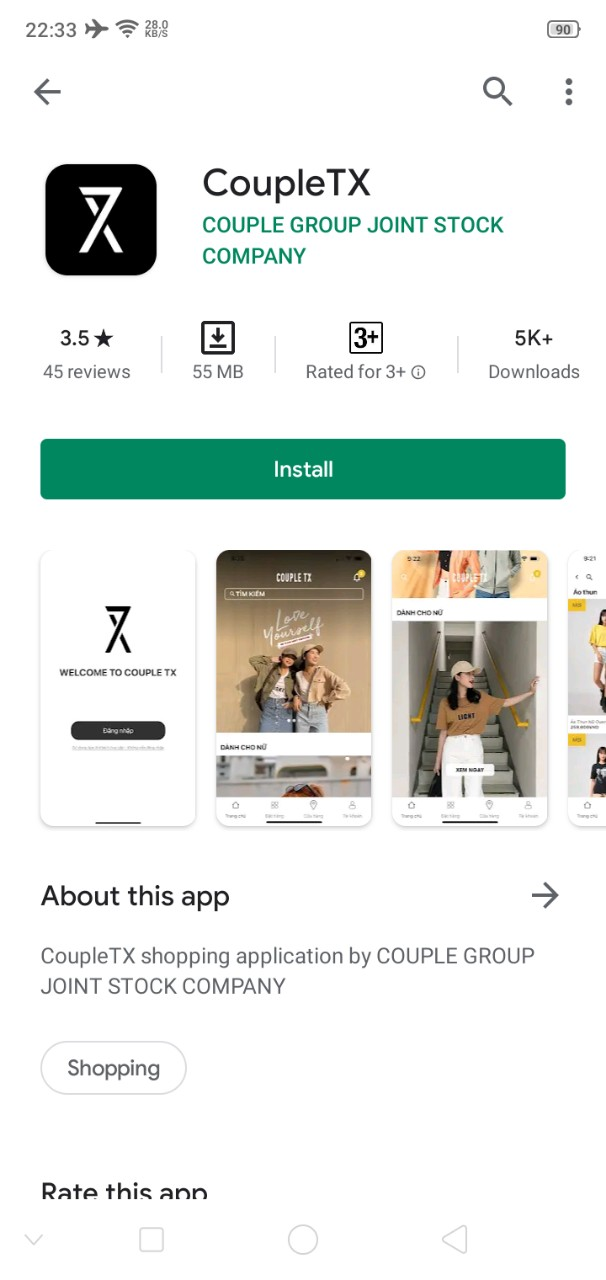
\includegraphics[height=10cm]{images/01.png}
    \caption{Ứng dụng CoupleTX trên GooglePlay}
\end{figure}

\indent và \textbf{Mr.Simple} - thời trang vest, blazer cho nam giới.

\begin{figure}[H]
    \centering
    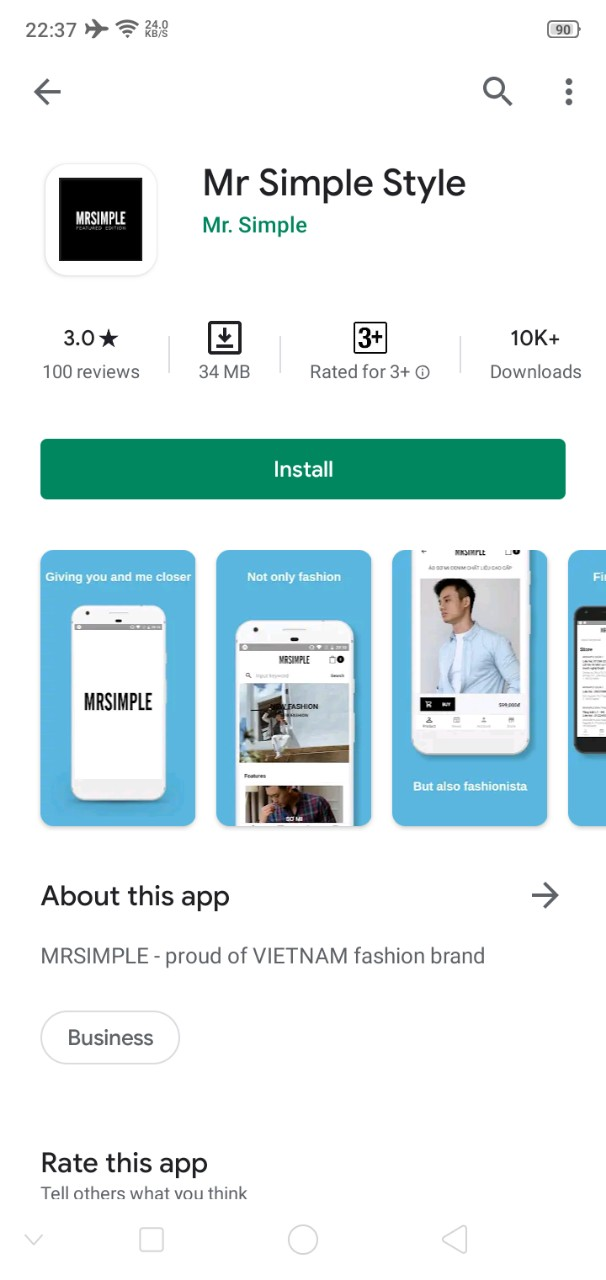
\includegraphics[height=10cm]{images/02.png}
    \caption{Ứng dụng Mr.Simple trên GooglePlay}
\end{figure}

\newpage
\indent Ngoài ra, ngoài phạm vị Việt Nam còn có ứng dụng mua sắm thời trang Farfetch.

\begin{figure}[H]
    \centering
    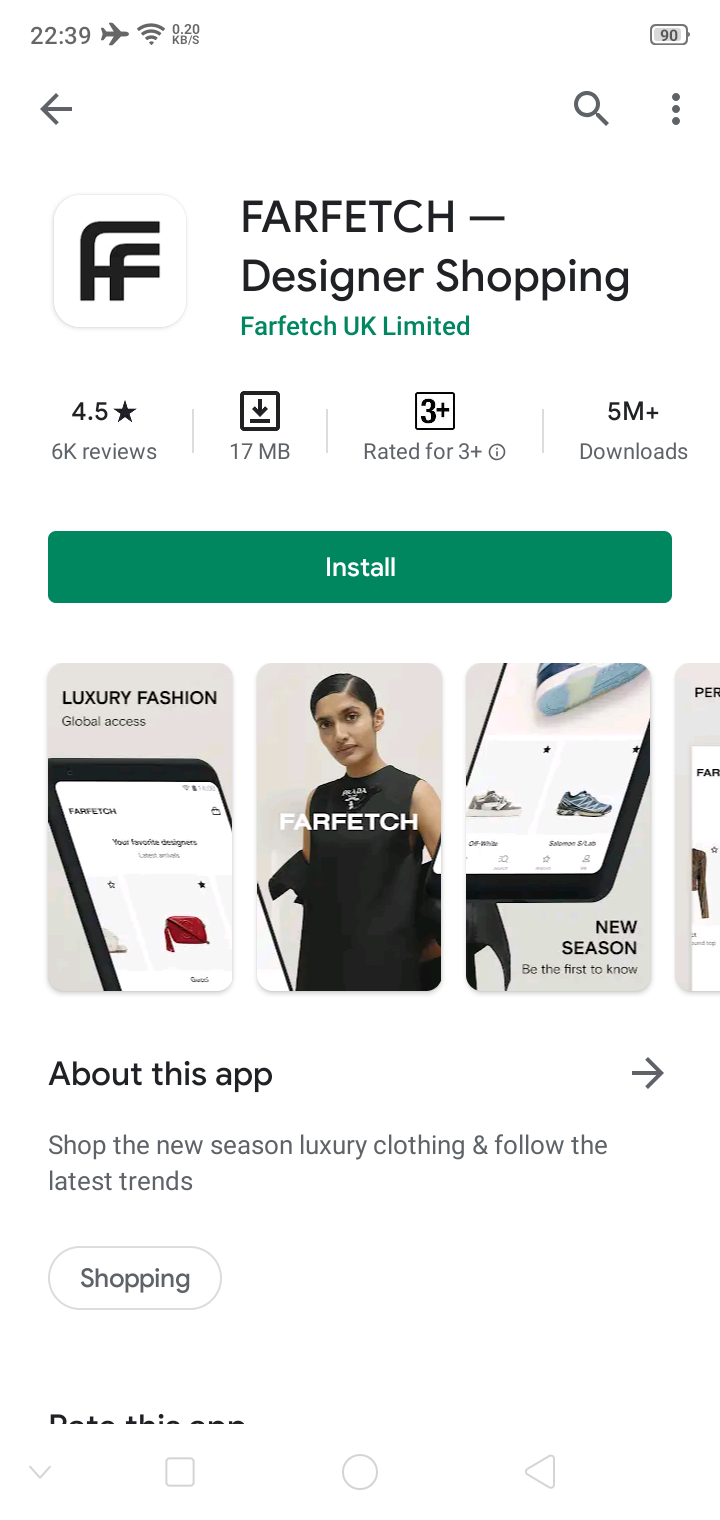
\includegraphics[height=10cm]{images/03.png}
    \caption{Ứng dụng Farfetch trên GooglePlay}
\end{figure}

\subsubsection{Điểm khác biệt của chương trình}
Không có.\\
\indent \textbf{Hạn chế}: Ứng dụng chỉ chạy ở phía client, không có web service nên một vài tính năng dù có trên front-end nhưng bên dưới backend thì chưa hỗ trợ và chưa có server.

\subsection{Đóng góp của các thành viên cho đồ án}
\subsubsection{Tỉ lệ đóng góp của các thành viên}
\begin{tabular}{ |p{1cm}||p{3cm}|p{6cm}|p{5cm}|  }
    \hline
    \textbf{STT} & \textbf{MSSV} & \textbf{Họ và tên}  & \textbf{Đóng góp} (tổng 100\%) \\
    \hline \hline
    1            & 19424915      & Dương Trọng Đức     & 30\%                           \\ \hline
    2            & 20424008      & Dương Mạnh Cường    & 36\%                           \\ \hline
    3            & 20424013      & Phạm Nguyễn Mỹ Diễm & 34\%                           \\
    \hline
\end{tabular}

\subsubsection{Chi tiết các công việc đã thực hiện}
\textbf{Lưu ý:} Các màn hình, tính năng mà nhóm đã đề cập ở báo cáo lần đầu nếu không có trong danh sách dưới đây thì là do nhóm chủ động dừng phát triển do không kiệp tiến độ thời gian môn học, phân bổ thời gian cho các thành viên trong nhóm để làm các đồ án môn học khác. Mong Thầy thông cảm cho nhóm.\\\\

\begin{tabular}{ |p{1cm}||p{3cm}|p{12cm}| }
    \hline
    \textbf{STT} & \textbf{SV thực hiện} & \textbf{Tên chức năng}                                                                                                                                 \\
    \hline \hline
    1            & 19424015              & Đăng ký tài khoản bằng email và password.                                                                                                              \\ \hline
    2            & 19424015              & Đăng nhập tài khoản bằng email và password.                                                                                                            \\ \hline
    3            & 19424015              & Đăng xuất tài khoản người dùng.                                                                                                                        \\ \hline
    4            & 19424015              & Khôi phục mật khẩu cho tài khoản bằng mail gửi đến cho email dùng để đăng ký tài khoản.                                                                \\ \hline
    5            & 19424015              & Màn hình cá nhân người dùng.                                                                                                                           \\ \hline
    6            & 20424008              & Màn hình chính của ứng dụng.                                                                                                                           \\ \hline
    7            & 20424008              & Màn hình splash-screen (trước đây được thực hiện bởi sinh viên 19424015 - sau này do sinh viên 20424008 chỉnh sửa thêm để phục vụ cho màn hình chính). \\ \hline
    8            & 20424008              & Màn hình sản phẩm yêu thích.                                                                                                                           \\ \hline
    9            & 20424008              & Chức năng tìm kiếm.                                                                                                                                    \\ \hline
    10           & 20424013              & Màn hình chi tiết sản phẩm.                                                                                                                            \\ \hline
    11           & 20424013              & Màn hình giỏ hàng.                                                                                                                                     \\ \hline
    12           & 20424013              & Màn hình thanh toán.                                                                                                                                   \\ \hline
    13           & 20424013              & Màn hình lịch sử đơn hàng.                                                                                                                             \\ \hline
\end{tabular}

\subsection{Thông tin cần thiết để chạy chương trình}
\textbf{Đối với ứng dụng sau khi release thành file *.apk}: Chỉ cần tải và cài đặt file \textsf{app-release.apk} trên thiết bị Android chạy Android 9.0 trở lên.\\

\textbf{Đối với giai đoạn phát triển:}
\begin{itemize}
    \item Cần được cấp quyền truy cập vào Firebase console từ trưởng nhóm để chỉnh sửa, thay đổi cài đặt các dịch vụ Firestore, Firestorage và Authentication.
    \item Android Emulator phải chạy Android 9.0 trở lên.
    \item Android Studio phải cài đặt SDK API 28.
\end{itemize}

\section{Các chức năng đã thực hiện}
Phần này sẽ mô tả chi tiết các công việc mà các thành viên của nhóm đã thực hiện trong mục 1.3.2. \textit{(vì để tiện cho việc trình bày, nhóm sẽ không trình bày theo thứ tự như đã liệt kê trong bảng, mong Thầy thông cảm)}.\\

\indent Dưới đây là logo của ứng dụng ở màn hình chính của thiết bị Anroid sau khi cài đặt \textit{(chú ý mũi tên màu đỏ)}.

\begin{figure}[H]
    \centering
    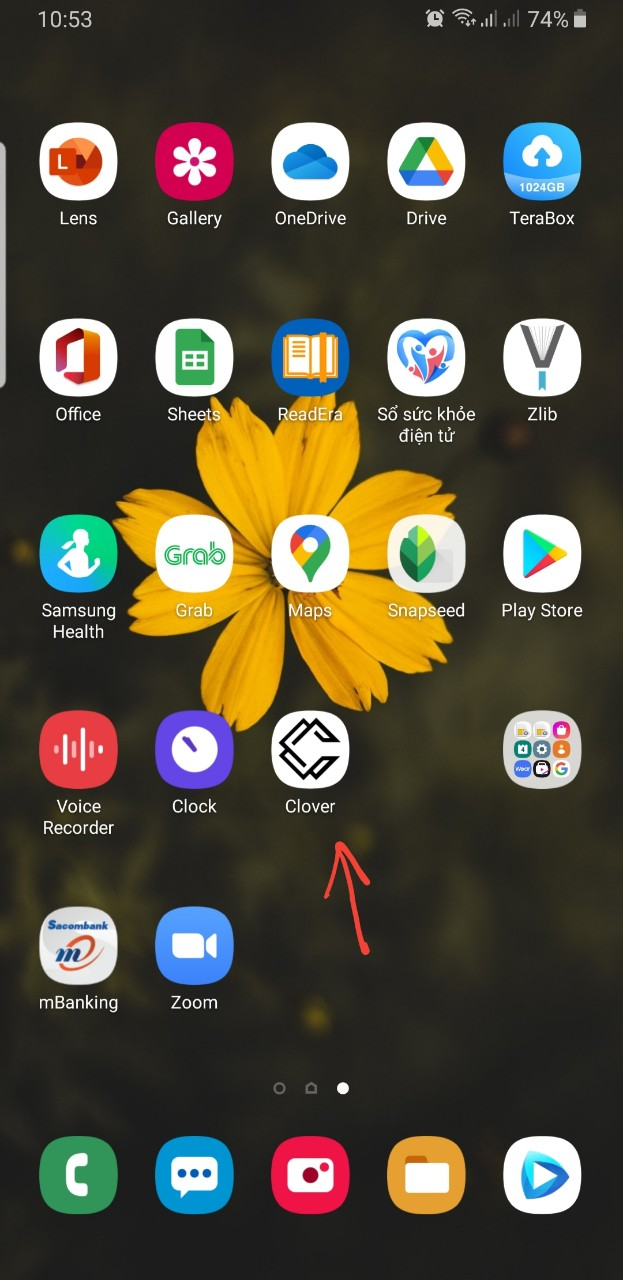
\includegraphics[height=10cm]{images/04.png}
    \caption{Logo của ứng dụng ở màn hình menu của thiết bị Android}
\end{figure}

\newpage
\subsection{Màn hình splash-screen}
Được thực hiện bởi sinh viên 20424008. Dưới đây là hình chụp của màn hình này.

\begin{figure}[H]
    \centering
    
\includegraphics[height=10cm]{images/05.png}
    \caption{Màn hình splash-screen}
\end{figure}

\indent Khi truy cập vào ứng dụng, người dùng sẽ gặp màn hình này đầu tiên.\\\\
\indent \textbf{Các thành phần và chức năng kèm theo trên màn hình}
\begin{itemize}
    \item Màn hình này sẽ hiển thị trong ba giây.
    \item Trong ba giây, back-end sẽ load dữ liệu như hình ảnh, tên sản phẩm, các custom icon của ứng dụng... từ Firestore về thiết bị để giảm tải cho màn hình chính. Người dùng cũng tránh việc có "cảm giác" phải chờ đợi.
    \item Kiểm tra người dùng là người dùng mới hay là người dùng cũ.
    
    \begin{itemize}
        \item Nếu là người dùng cũ thì sẽ đi thẳng đến màn hình chính của ứng dụng.
        \item Nếu là người dùng mới (người dùng cũ nhưng đã đăng xuất tài khoản, người dùng vừa cài ứng dụng lên thiết bị,...) thì sẽ đi thẳng đến màn hình đăng nhập.
    \end{itemize}
\end{itemize}

\subsection{Màn hình đăng nhập}
\subsubsection{Chức năng đăng nhập}
Được thực hiện bởi sinh viên 19424015. Dưới đây là hình chụp của màn hình này.\\

\indent Chức năng đăng nhập này sử dụng dịch vụ Firebase Authentication của Google cung cấp.\\

\indent Người dùng sẽ được đưa đến màn hình này khi:
\begin{itemize}
    \item Là người dùng cũ nhưng đã đăng xuất tài khoản.
    \item Là người dùng mới (vừa cài đặt ứng dụng).
    \item Người dùng bỏ qua bước đăng nhập đi thẳng vào màn hình chính nhưng về sau lại có nhu cầu đăng nhập để đặt hàng, thanh toán,... và được màn hình chính đưa lại về đây. 
\end{itemize}

\begin{figure}[H]
    \centering
    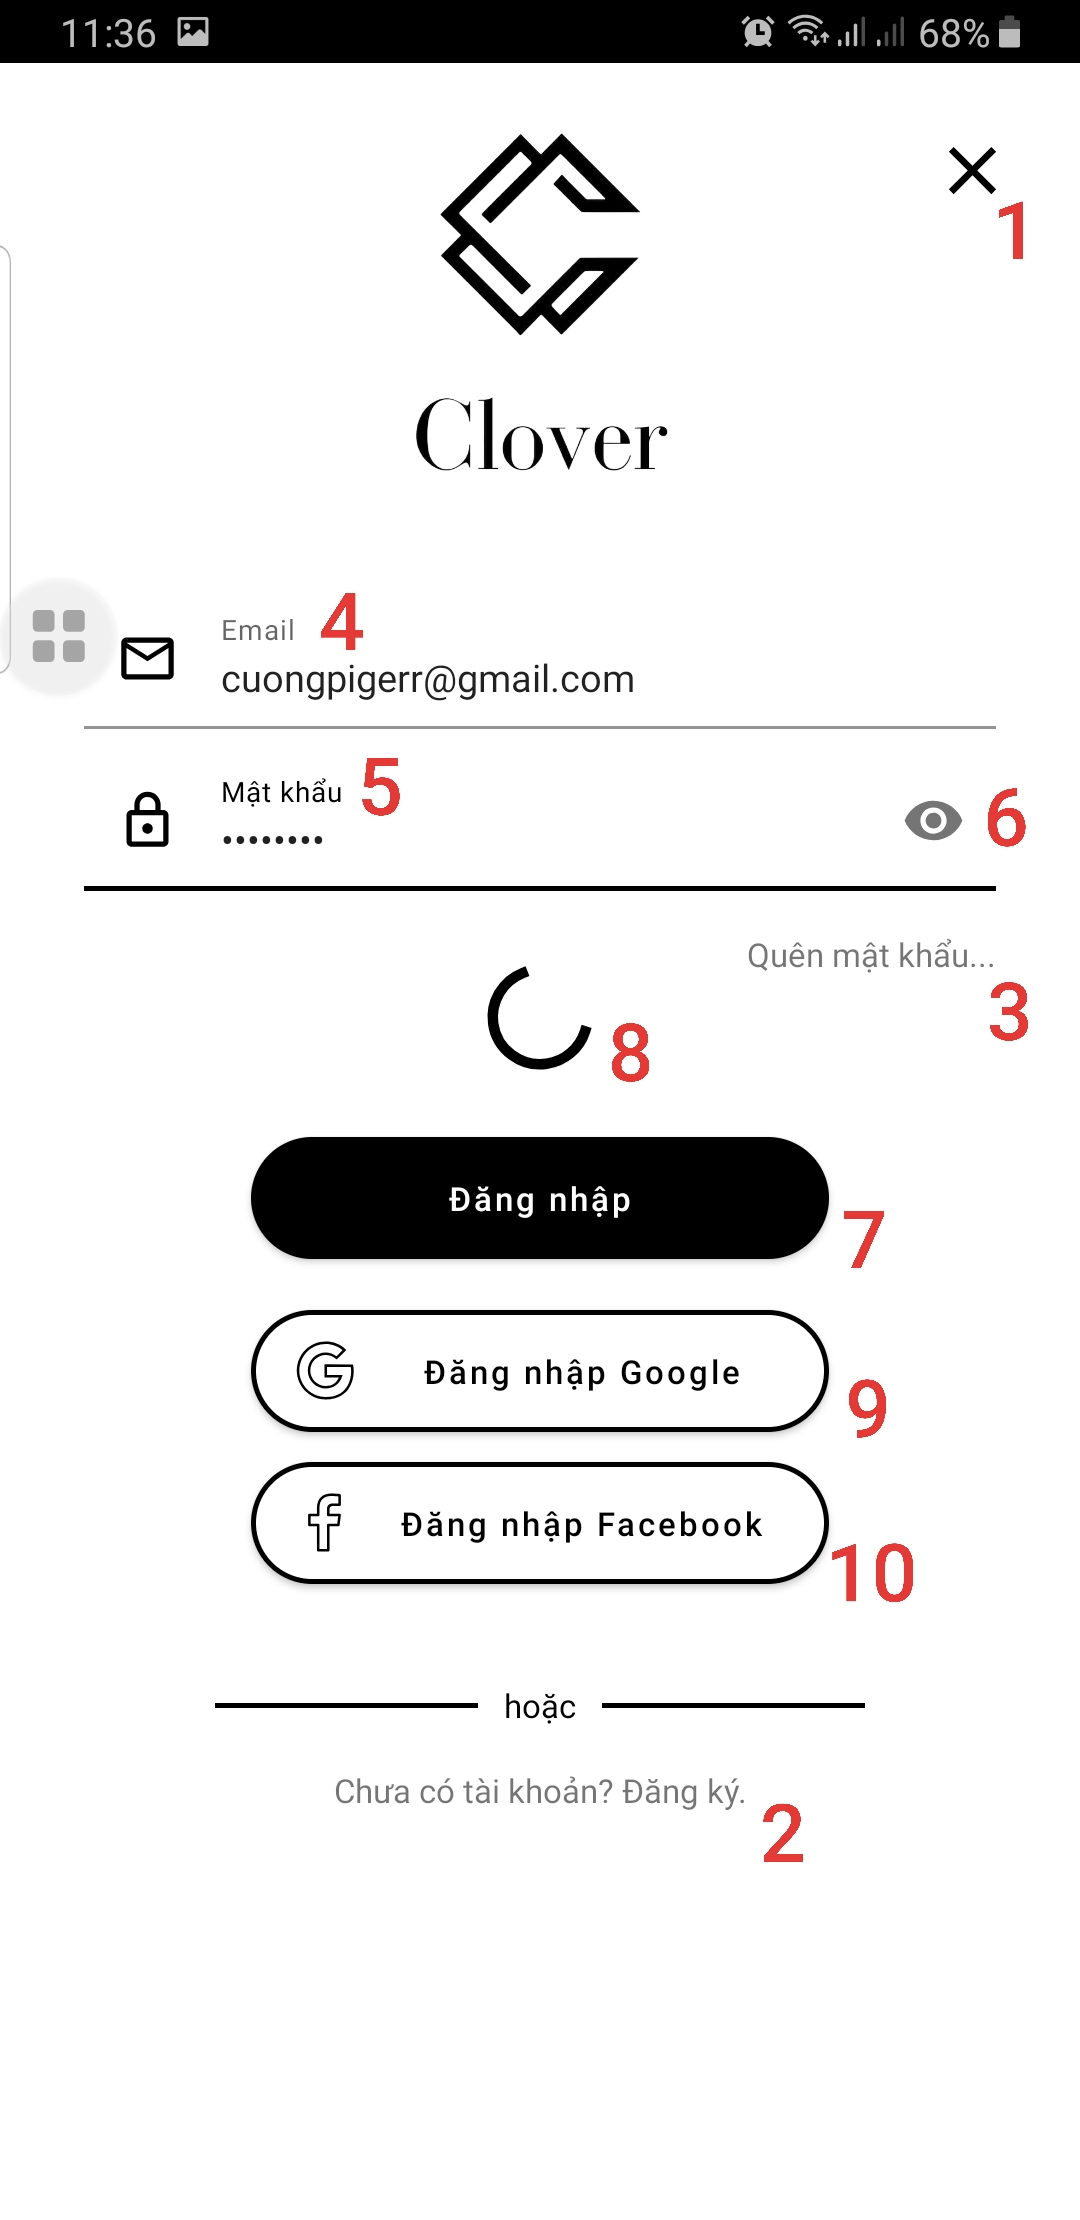
\includegraphics[height=10cm]{images/06.png}
    \caption{Màn hình đăng nhập - chức năng đăng nhập}
\end{figure}

\indent \textbf{Các thành phần và chức năng kèm theo trên màn hình}
\begin{itemize}
    \item \textbf{1}: Image button - khi nhấn vào button này người dùng sẽ được chuyển thẳng đến màn hình chính của ứng dụng mà \textbf{không cần đăng nhập}.
    \item \textbf{2}: Text button - khi nhấn vào sẽ đưa đến fragment đăng ký tài khoản mới cho người dùng ở mục 2.2.3.
    \item \textbf{3}: Text button - khi nhấn vào đưa người dùng đến fragment đặt lại mật khẩu ở mục 2.2.2.
    \item \textbf{4}: Text input layout: nhập thông tin email của người dùng. Trong quá trình người dùng typing - thực hiện kiểm tra hợp lệ để thông báo ngay cho người dùng biết.
    \item \textbf{5}: Text input layout: nhập mật khẩu của người dùng.
    \item \textbf{6}: Icon - Khi nhấn vào sẽ hiển thị mật khẩu ở \textbf{5} ra dưới dạng text.
    \newpage
    \item \textbf{7}: Button - khi nhấn vào sẽ lấy thông tin ở \textbf{4} và \textbf{5} $\Rightarrow$  kiểm tra hợp lệ (nếu không hợp lệ sẽ thông báo ngay trên Text input layout của \textbf{4} và \textbf{5}) $\Rightarrow$ nếu hợp lệ, đăng nhập vào ứng dụng thông qua Firebase Authentication, sau đó sẽ bị deactive cho đến khi Firebase Authentication xử lý xong.
    \begin{itemize}
        \item \textbf{Nếu thành công}: Người dùng được chuyển thẳng đến màn hình chính của ứng dụng.
        \item \textbf{Nếu thất bại}: Hiển thị một Alert Dialog thông báo cho người dùng biết là đăng nhập thất bại.
    \end{itemize}
    \item \textbf{8}: Progress Circle - luôn ẩn đi, chỉ hiển thị khi người dùng nhấn vào \textbf{7} để cho người dùng biết rằng hệ thống vẫn chạy và đang trong quá trình kiểm tra đăng nhập.
    \item \textbf{9}: Button - dùng để đăng nhập qua Google nhưng chỉ mới có ở front-end, back-end vẫn chưa thực hiện do không kịp tiến độ môn học.
    \item \textbf{10}: Button - dùng để đăng nhập qua Facebook nhưng chỉ mới có ở front-end, back-end vẫn chưa thực hiện do không kịp tiến độ môn học.
\end{itemize}

\subsubsection{Chức năng đặt lại mật khẩu}
Được thực hiện bởi sinh viên 19424015. Dưới đây là hình chụp của màn hình này.\\

\indent Chức năng đặt lại mật khẩu sử dụng Firebase Authentication để gửi mail kèm theo link đặt lại password về cho email mà người dùng dùng để đăng nhập tài khoản.\\

\indent Người dùng sẽ được đưa về fragment này sau khi nhấn vào thành phần \textbf{3} trên fragment đăng nhập ở mục 2.2.1.

\begin{figure}[H]
    \centering
    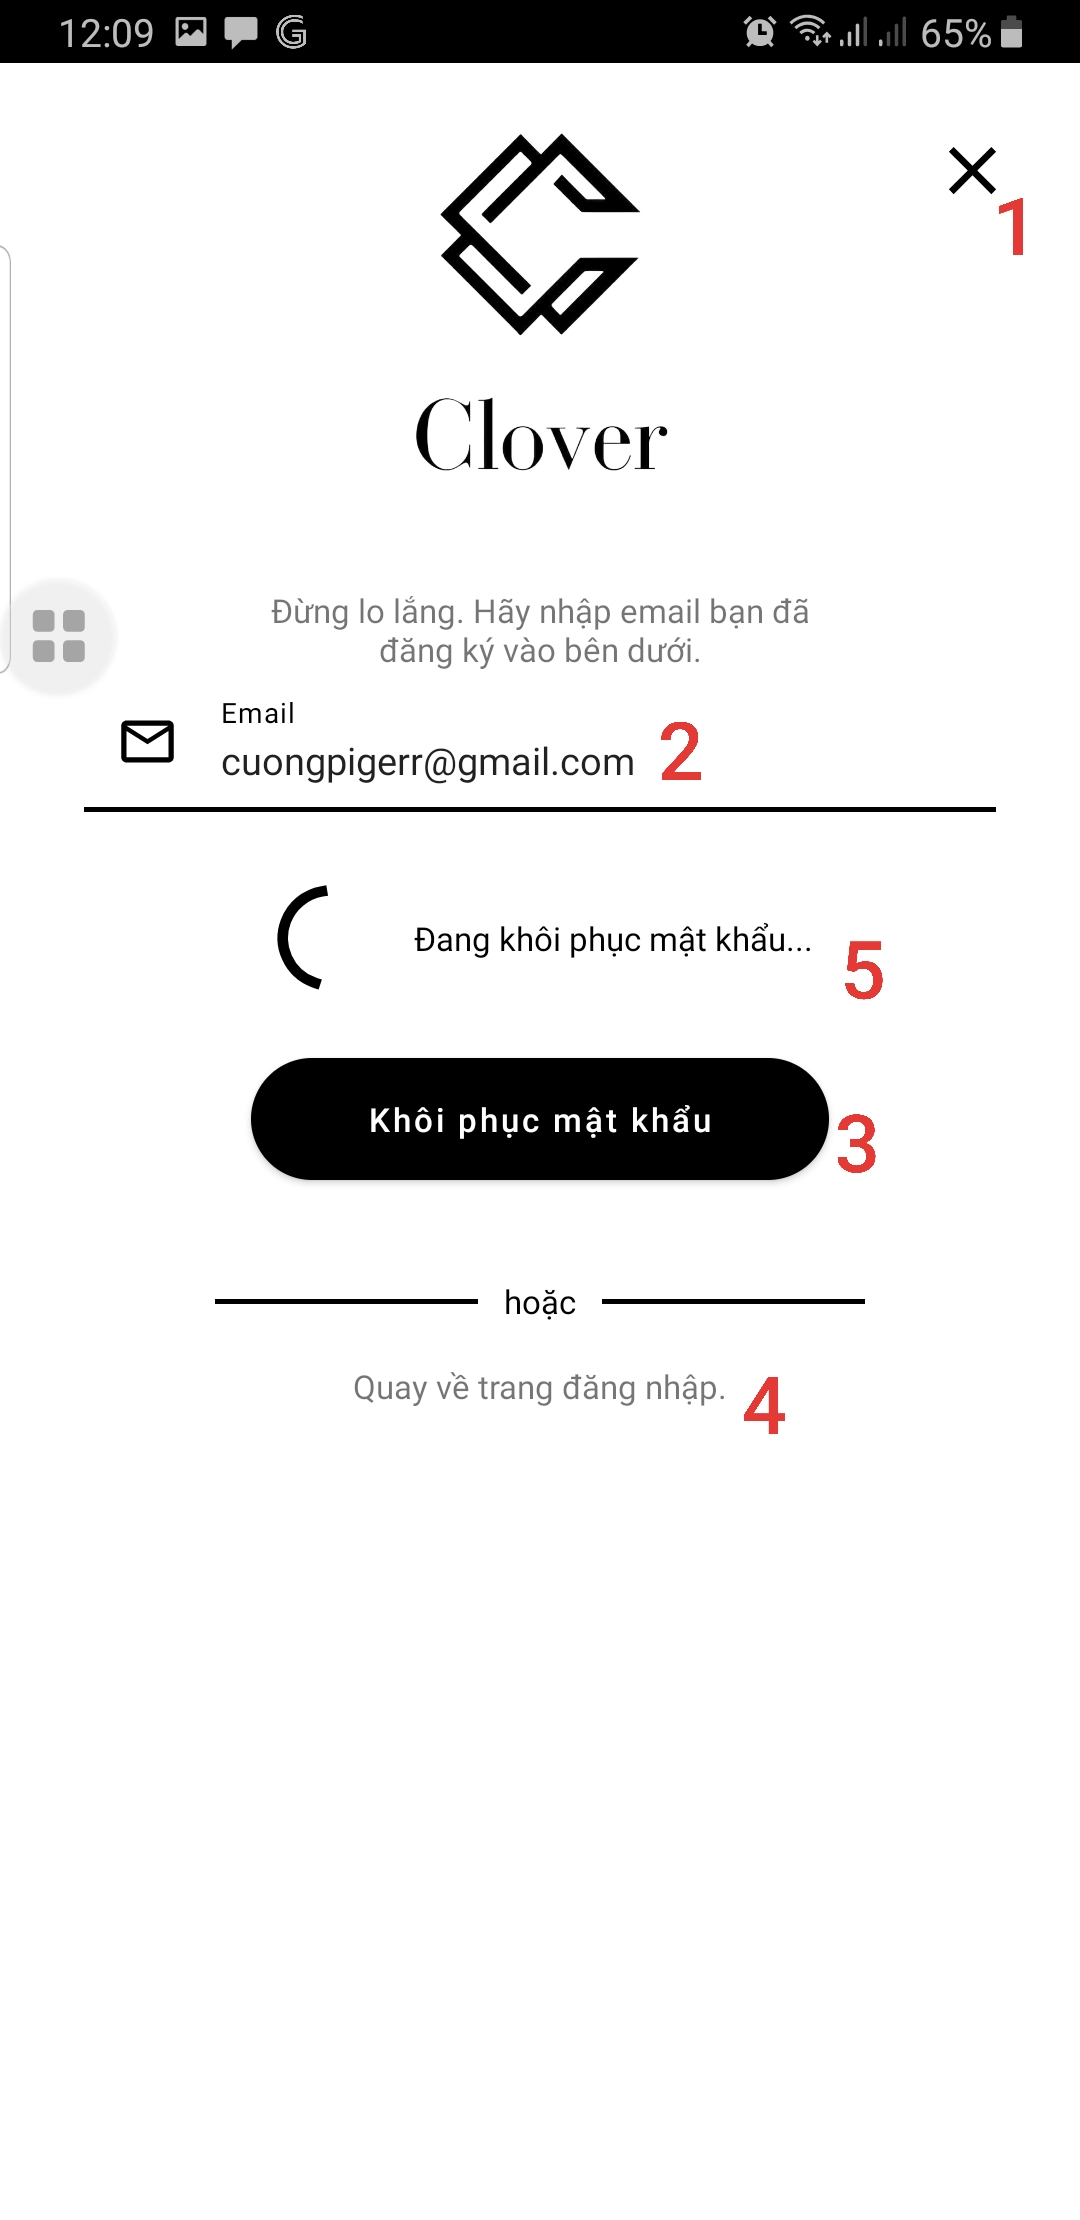
\includegraphics[height=10cm]{images/07.png}
    \caption{Màn hình đặt lại mật khẩu - nhập thông tin}
\end{figure}

\begin{figure}[H]
    \centering
    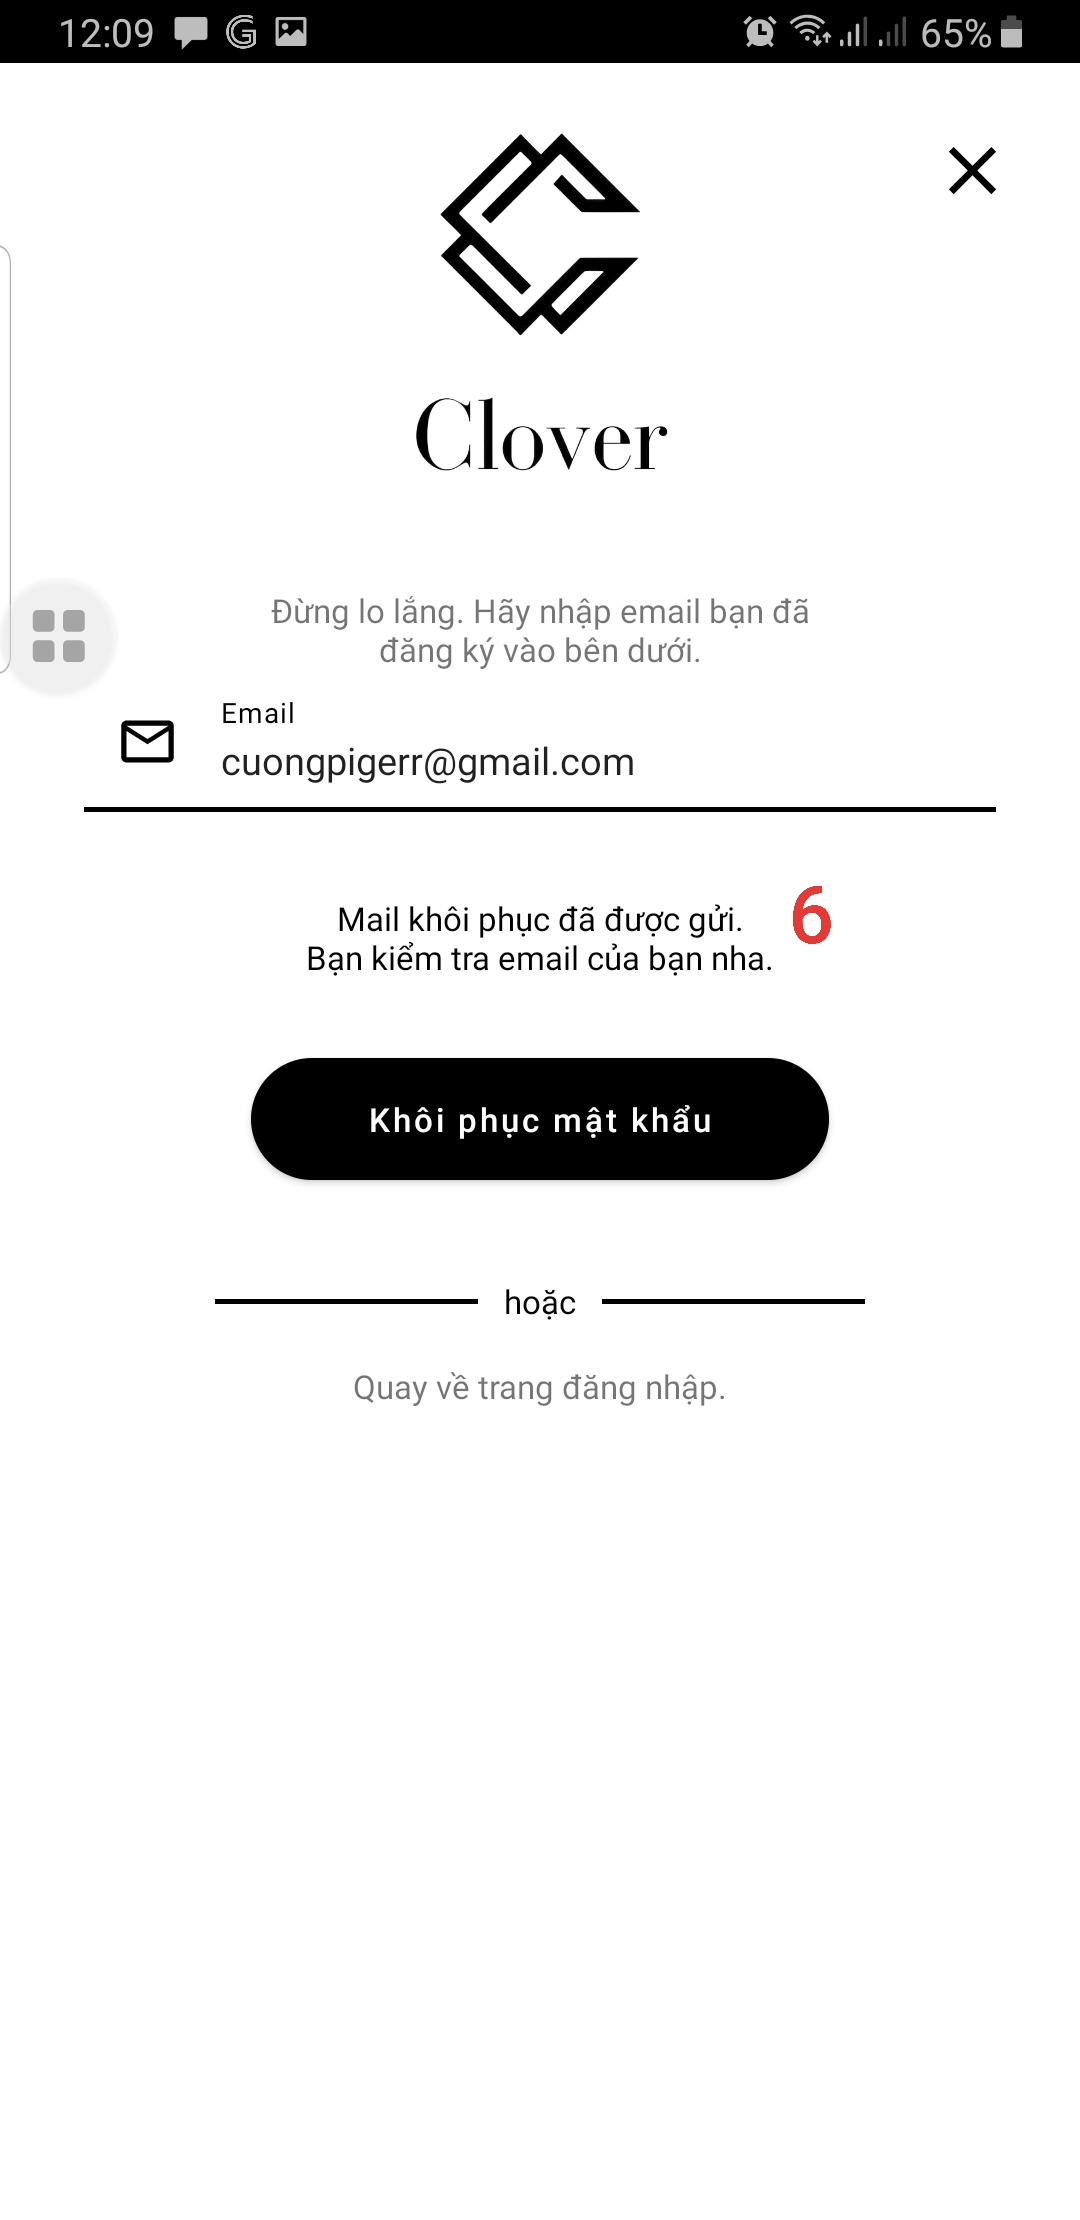
\includegraphics[height=10cm]{images/08.png}
    \caption{Màn hình đặt lại mật khẩu - thông báo cho người dùng biết đã gửi mail thành công}
\end{figure}

\begin{figure}[H]
    \centering
    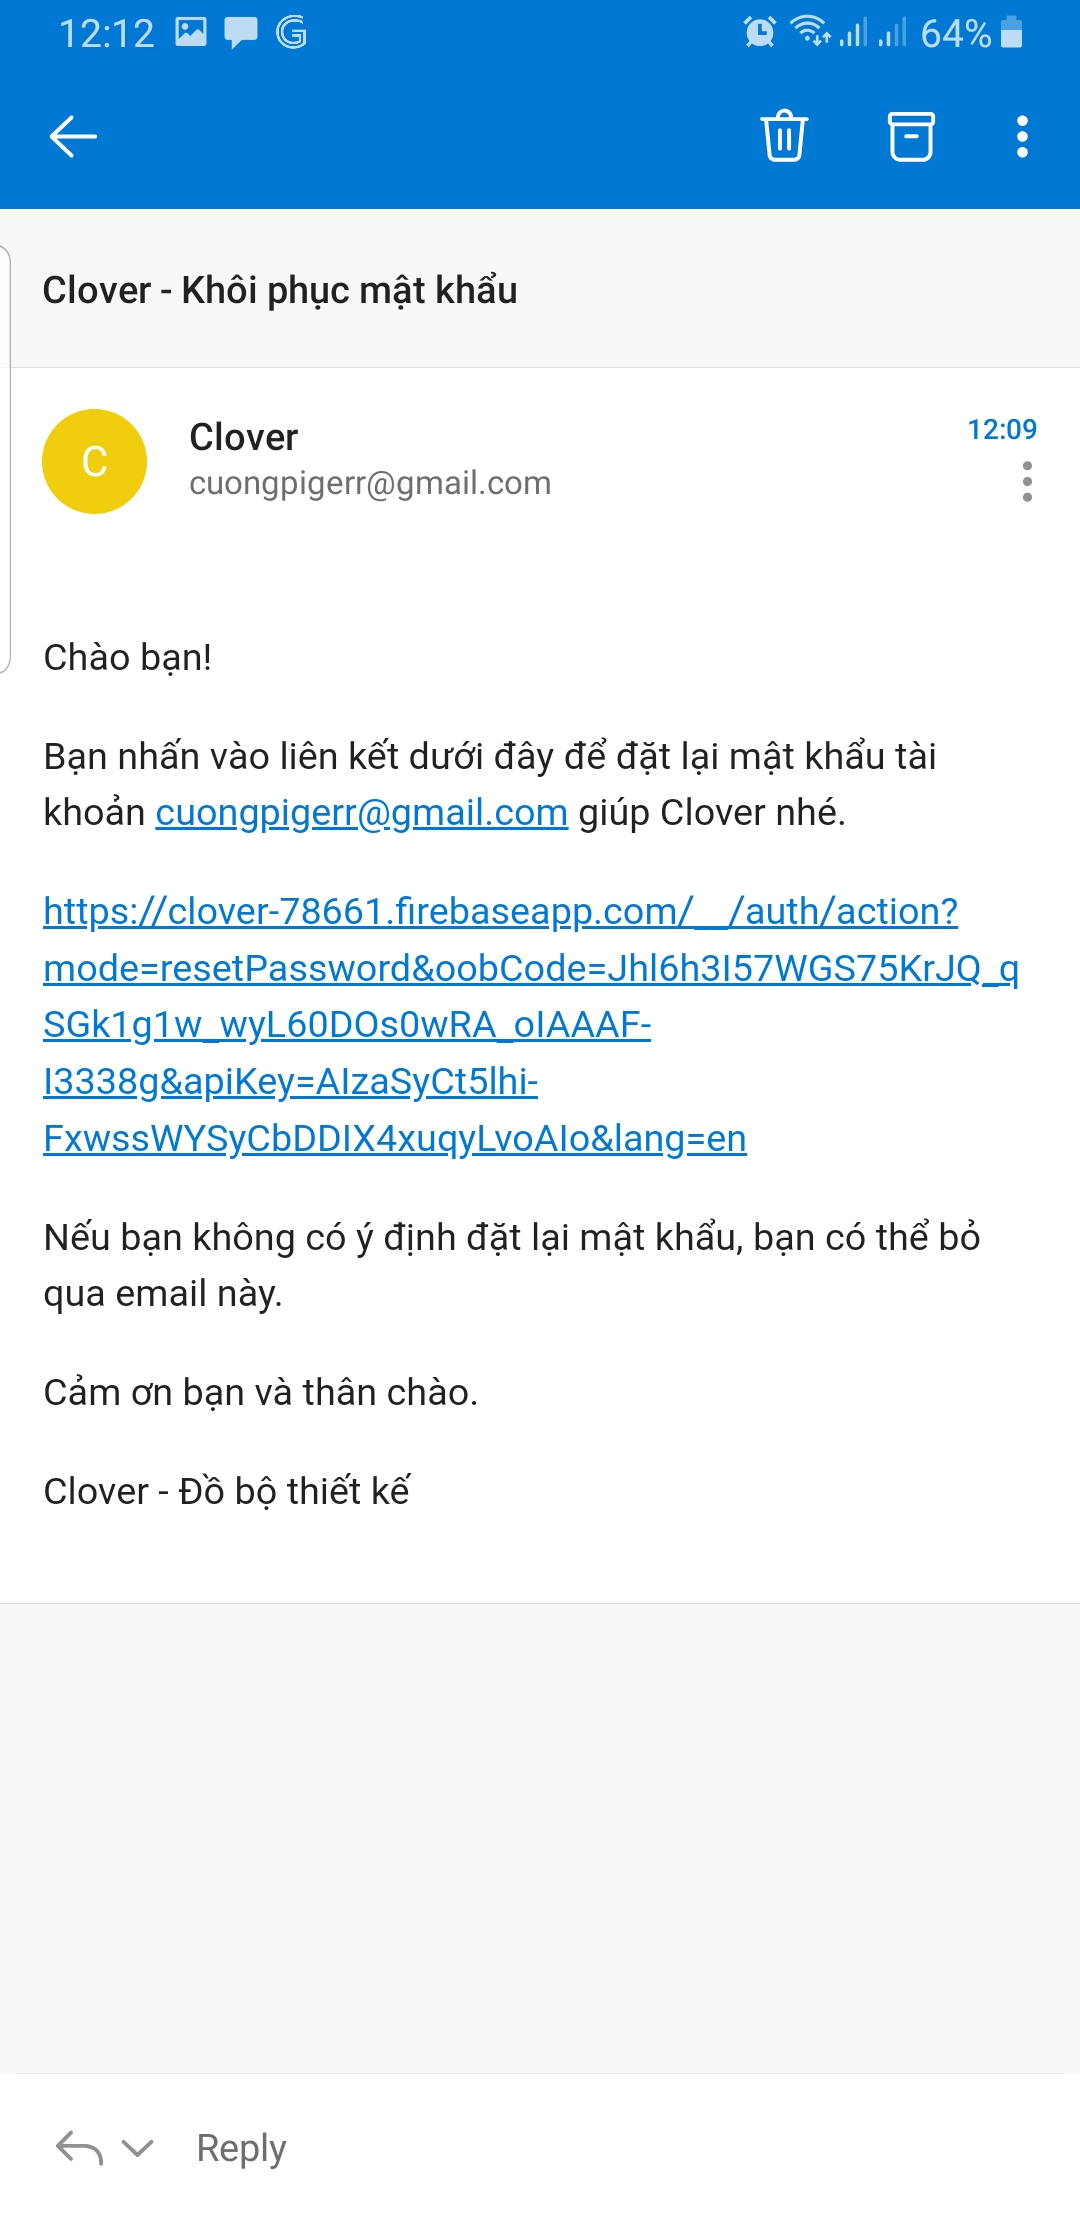
\includegraphics[height=10cm]{images/09.png}
    \caption{Mail khôi phục kèm link đặt lại mật khẩu được gửi về cho email mà người dùng dùng để đăng nhập tài khoản}
\end{figure}

\indent \textbf{Các thành phần và chức năng kèm theo trên màn hình}
\begin{itemize}
    \item \textbf{1}: Image button - nhấn vào để đi thẳng đến màn hình chính của ứng dụng mà không cần đăng nhập.
    \item \textbf{2}: Text input layout - nhập email mà người dùng muốn đặt lại mật khẩu.
    \item \textbf{3}: Button - nhấn vào để gửi mail đặt lại mật khẩu.
    \item \textbf{4}: Text button - nhấn vào để trở về chức năng đăng nhập ở mục 2.2.1.
    \item \textbf{5}: Progress circle + Text view: cho người dùng biết mail khôi phục mật khẩu đang được gửi đến email được cung cấp ở \textbf{2}.
    \item \textbf{6}: Text view - cho người dùng biết đã gửi mail thành công.
\end{itemize}

\subsubsection{Chức năng đăng ký tài khoản}
Được thực hiện bởi sinh viên 19424015. Dưới đây là hình chụp của màn hình này.\\

\indent Chức năng đăng ký tài khoản sử dụng Firebase Authentication để đăng ký tài khoản cho người dùng.\\

\indent Người dùng sẽ được đưa thẳng đến fragment này sau khi nhấn vào thành phần \textbf{2} trên fragment đăng nhập ở mục 2.2.1.

\begin{figure}[H]
    \centering
    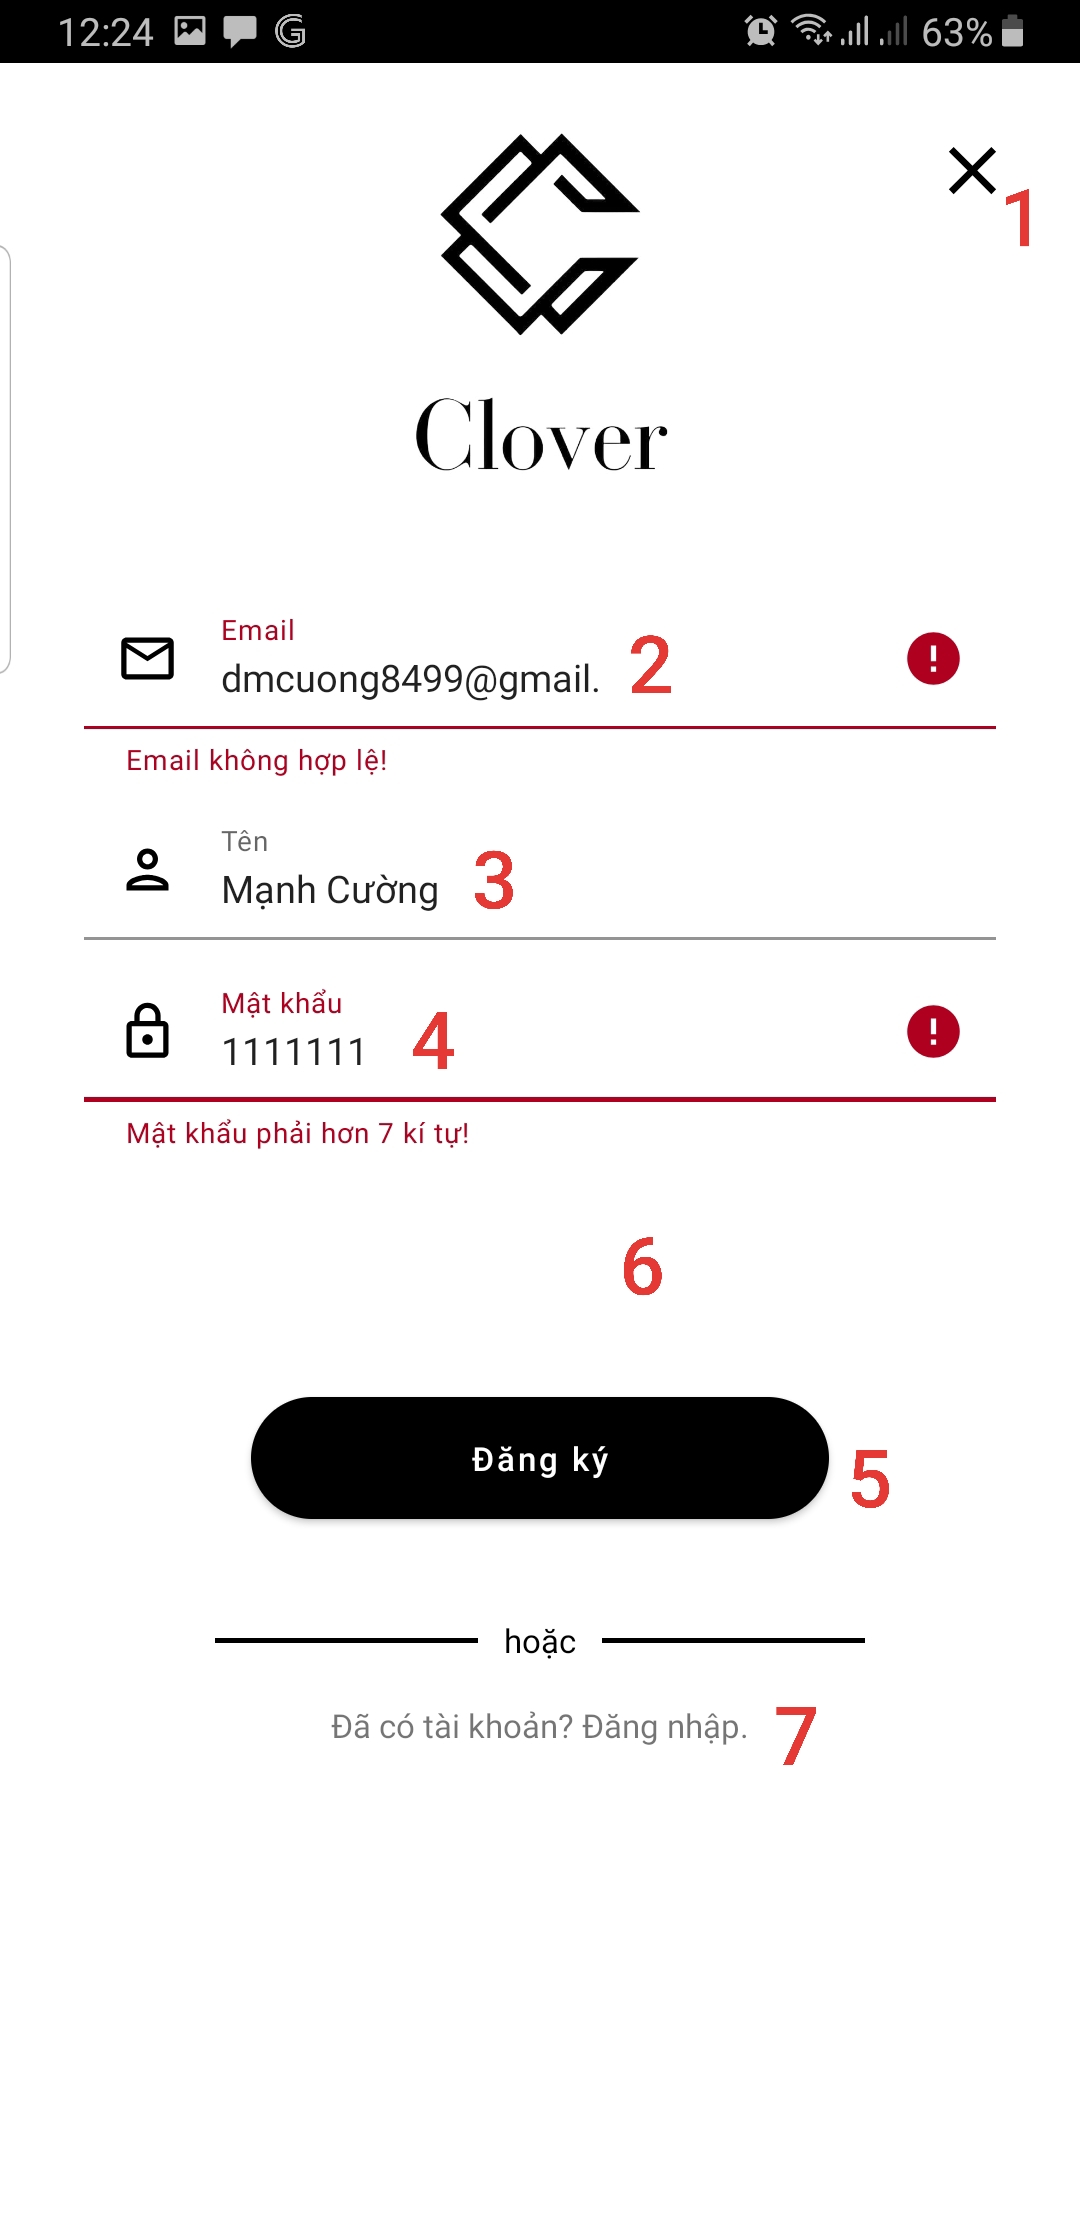
\includegraphics[height=10cm]{images/10.png}
    \caption{Màn hình đăng ký tài khoản}
\end{figure}

\indent \textbf{Các thành phần và chức năng kèm theo trên màn hình}
\begin{itemize}
    \item \textbf{1}: Image button - nhấn vào để đi thẳng đến màn hình chính của ứng dụng mà không cần đăng nhập.
    \item \textbf{2}: Text input layout - nhập email mà người dùng muốn tạo tài khoản (ở đây nhóm cố tình nhập sai định dạng email để Thầy có thể thấy được là ứng dụng có kiểm tra hợp lệ của các trường dữ liệu).
    \item \textbf{3}: Text input layout - nhập tên cho người dùng.
    \item \textbf{4}: Text input layout - nhập mật khẩu cho người dùng (ở đây nhóm cố tình nhập nhập password không hợp lệ để Thầy có thể thấy được là ứng dụng có kiểm tra hợp lệ của các trường dữ liệu).
    \item \textbf{5}: Button - khi nhấn vào, ứng dụng có hai khả năng trả về:
    \begin{itemize}
        \item \textbf{Thành công}: người dùng được đưa thẳng đến màn hình chính của ứng dụng và được Firestore ghi lại các thông tin của người dùng thành một document bên trong collection \textsf{UserModel} (nhóm sẽ trình bày sau).
        \item \textbf{Thất bại}: do email này đã được đăng ký trước đó hoặc vì một nguyên nhân nào đó $\Rightarrow$ hiển thị AlertDialog thông báo cho người dùng biết đăng ký thất bại.
    \end{itemize}

    \newpage
    \item \textbf{6}: Progress circle - về hình ảnh như các progress circle ở fragment đăng nhập + fragment đặt lại mật khẩu và luôn ẩn đi, chỉ hiển thị khi người dùng nhấn vào \textbf{5} (ở đây không hiển thị là do em chưa nhấn vào thành phần \textbf{5} và cũng không thể nhấn vào do \textbf{2} + \textbf{4} vi phạm trường dữ liệu).
    \item \textbf{7}: Image button - nhấn vào sẽ dược chuyển về chức năng đăng nhập ở mục 2.2.1.
\end{itemize}

\subsection{Màn hình chính}
Được thực hiện bởi sinh viên 20424008.\\

\indent Màn hình này được đưa đến khi:
\begin{itemize}
    \item Người dùng nhấn vào thành phần \textbf{1} ở các mục 2.2.1, 2.2.2 và 2.2.3.
    \item Người dùng đăng nhập thành công ở mục 2.2.1.
    \item Người dùng đăng ký tài khoản thành công ở mục 2.2.3.
\end{itemize}

\subsubsection{Màn hình trang chủ}
Được thực hiện bởi sinh viên 20424008. Dưới đây là hình chụp của màn hình này.\\

\begin{figure}[H]
    \centering
    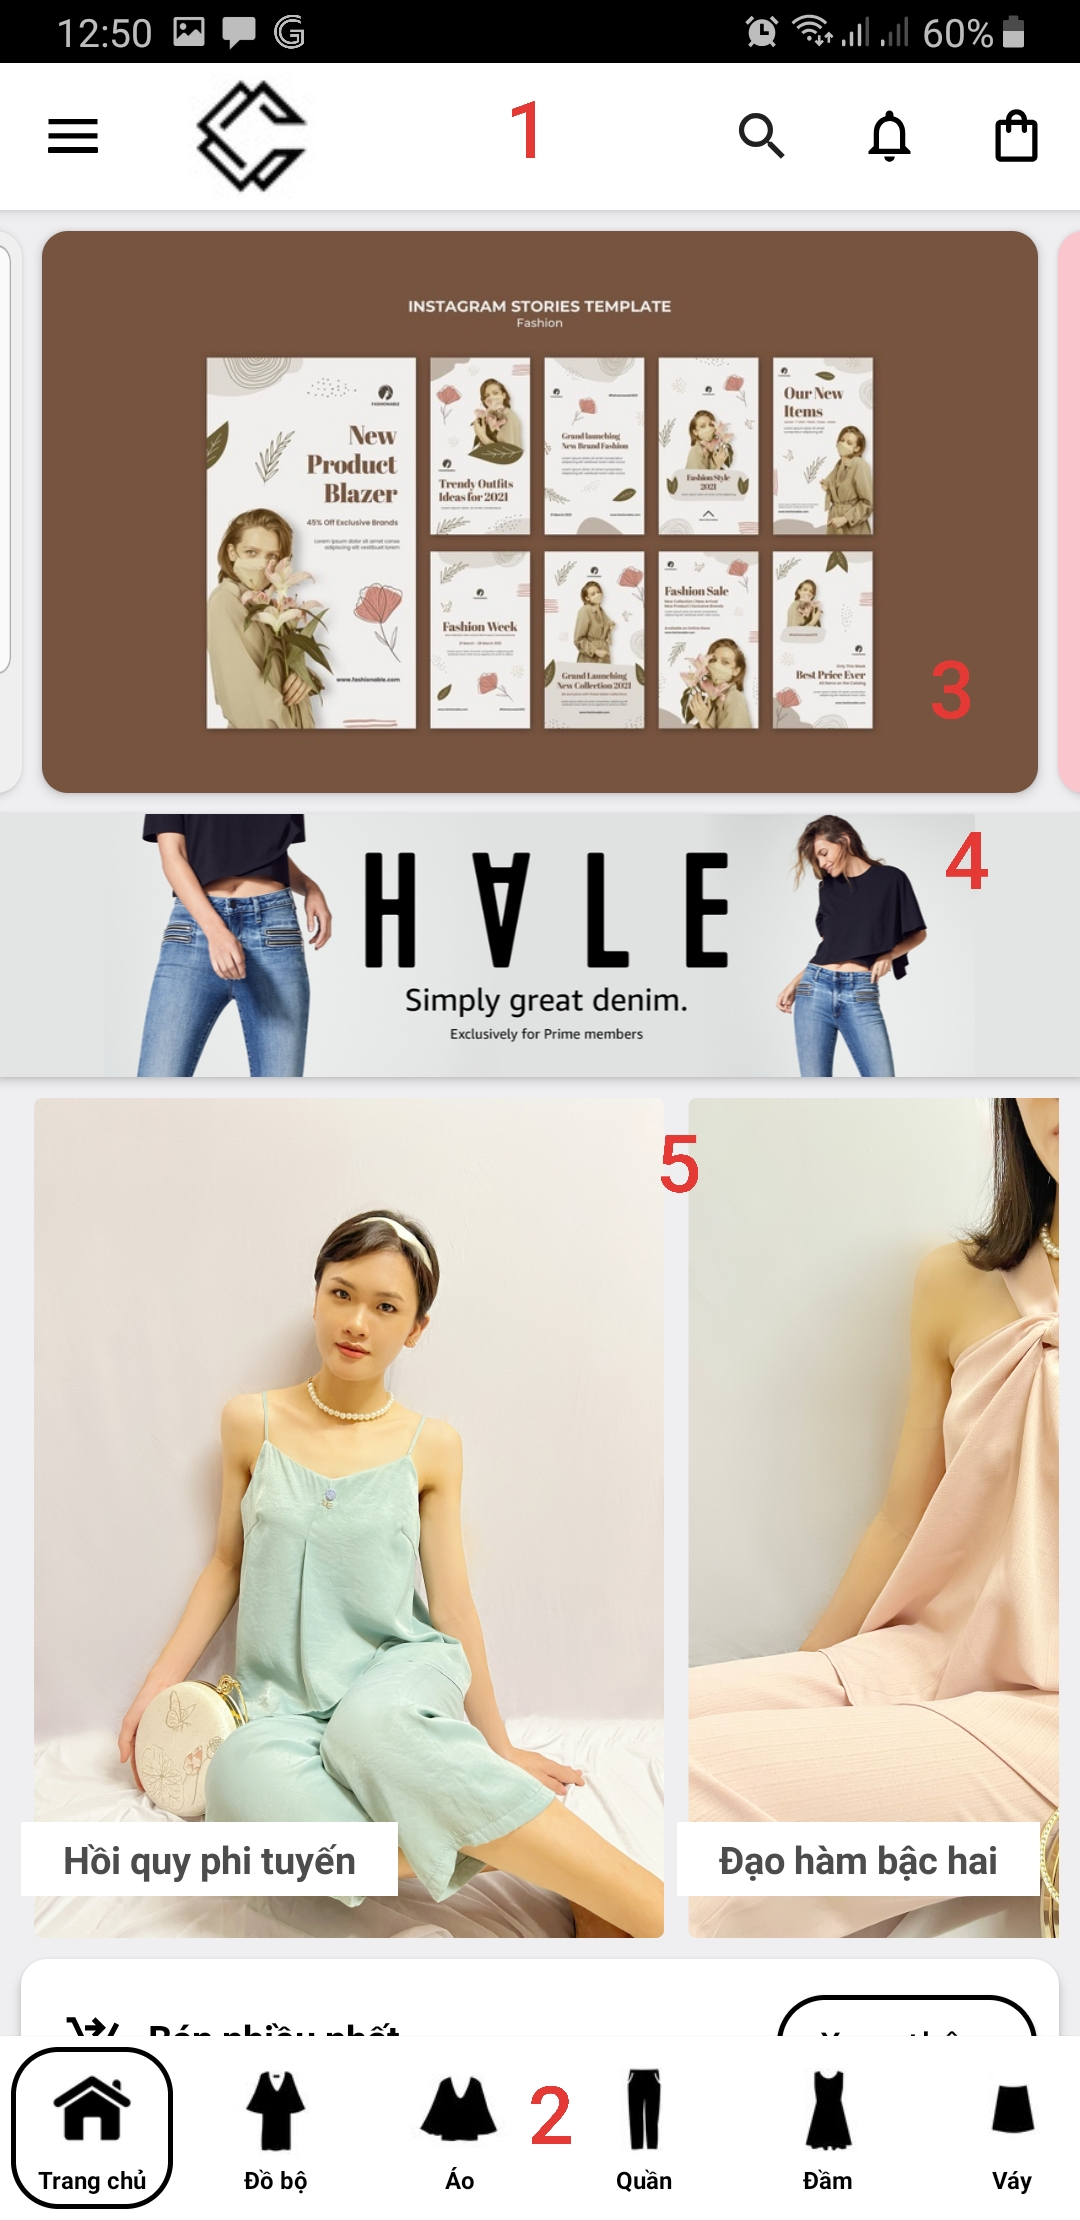
\includegraphics[height=10cm]{images/11.png}
    \caption{Màn hình trang chủ 1}
\end{figure}

\newpage
\indent \textbf{Các thành phần và chức năng kèm theo trên màn hình (1)}
\begin{itemize}
    \item \textbf{1}: Action bar - chứa các thành phần từ trái qua phải như sau:
    \begin{itemize}
        \item Hamburger toggle - nhấn vào để mở navigation view.
        \item Actionbar logo - hiển thị logo của ứng dụng.
        \item Menu item Search - chức năng tìm kiếm.
        \item Menu item Notification - chức năng thông báo (chưa hỗ trợ do ứng dụng chưa có web service + server xử lí).
        \item Menu item Cart - bấm vào để đi đến fragment giỏ hàng.
    \end{itemize}

    \item \textbf{2}: Horizontal Recycler View - hiển thị các sản phẩm theo danh mục.
    \item \textbf{3}: Carousel (Horizontal Recycler View) - hiển thị các chương trình, khuyến mãi của cửa hàng. Sau ba giây sẽ tự chuyển.
    \item \textbf{4}: Banner (Image View) - dùng để chèn quảng cáo.
    \item \textbf{5}: Slider (Horizontal Recycler View) - hiển thị các sản phẩm mới nhất. Nhấn vào item sẽ đưa đến trang chi tiết sản phẩm tương ứng, fragment này được trình bày trong mục 2.3.4.
\end{itemize}

\newpage
\begin{figure}[H]
    \centering
    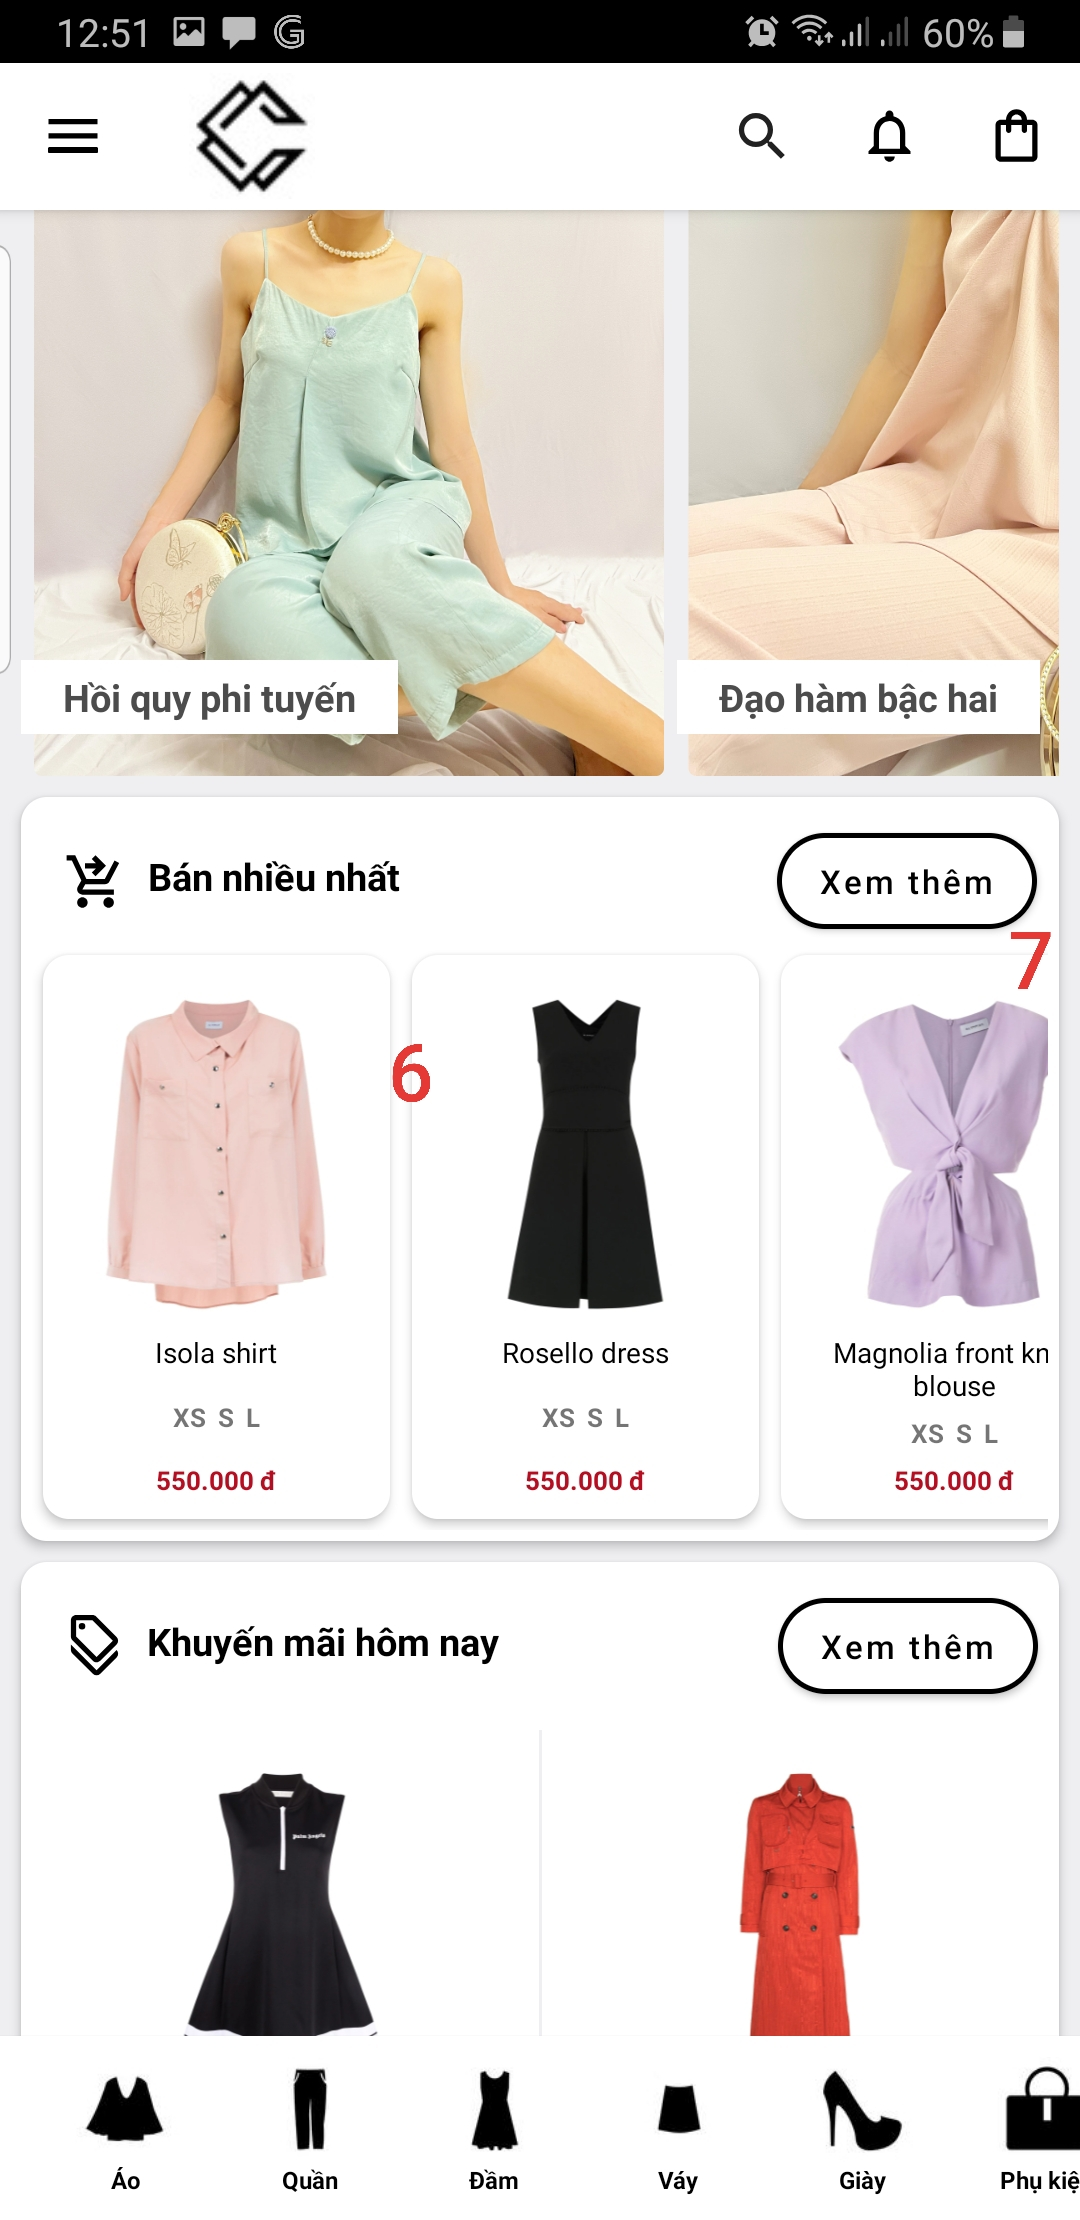
\includegraphics[height=10cm]{images/12.png}
    \caption{Màn hình trang chủ 2}
\end{figure}

\indent \textbf{Các thành phần và chức năng kèm theo trên màn hình (2)}
\begin{itemize}
    \item \textbf{6}: Horizontal Recycler View - hiển thị tám các sản phẩm bán chạy hiện tại. Nhấn vào item sẽ đưa đến trang chi tiết sản phẩm tương ứng, fragment này sẽ trình bày trong mục 2.3.4.
    \item \textbf{7}: Button - đưa đến một fragment khác hiển thị nhiều hơn tám sản phẩm bán chạy dưới dạng GridView, fragment này sẽ được trình bày ở mục 2.3.2.
\end{itemize}

\newpage
\begin{figure}[H]
    \centering
    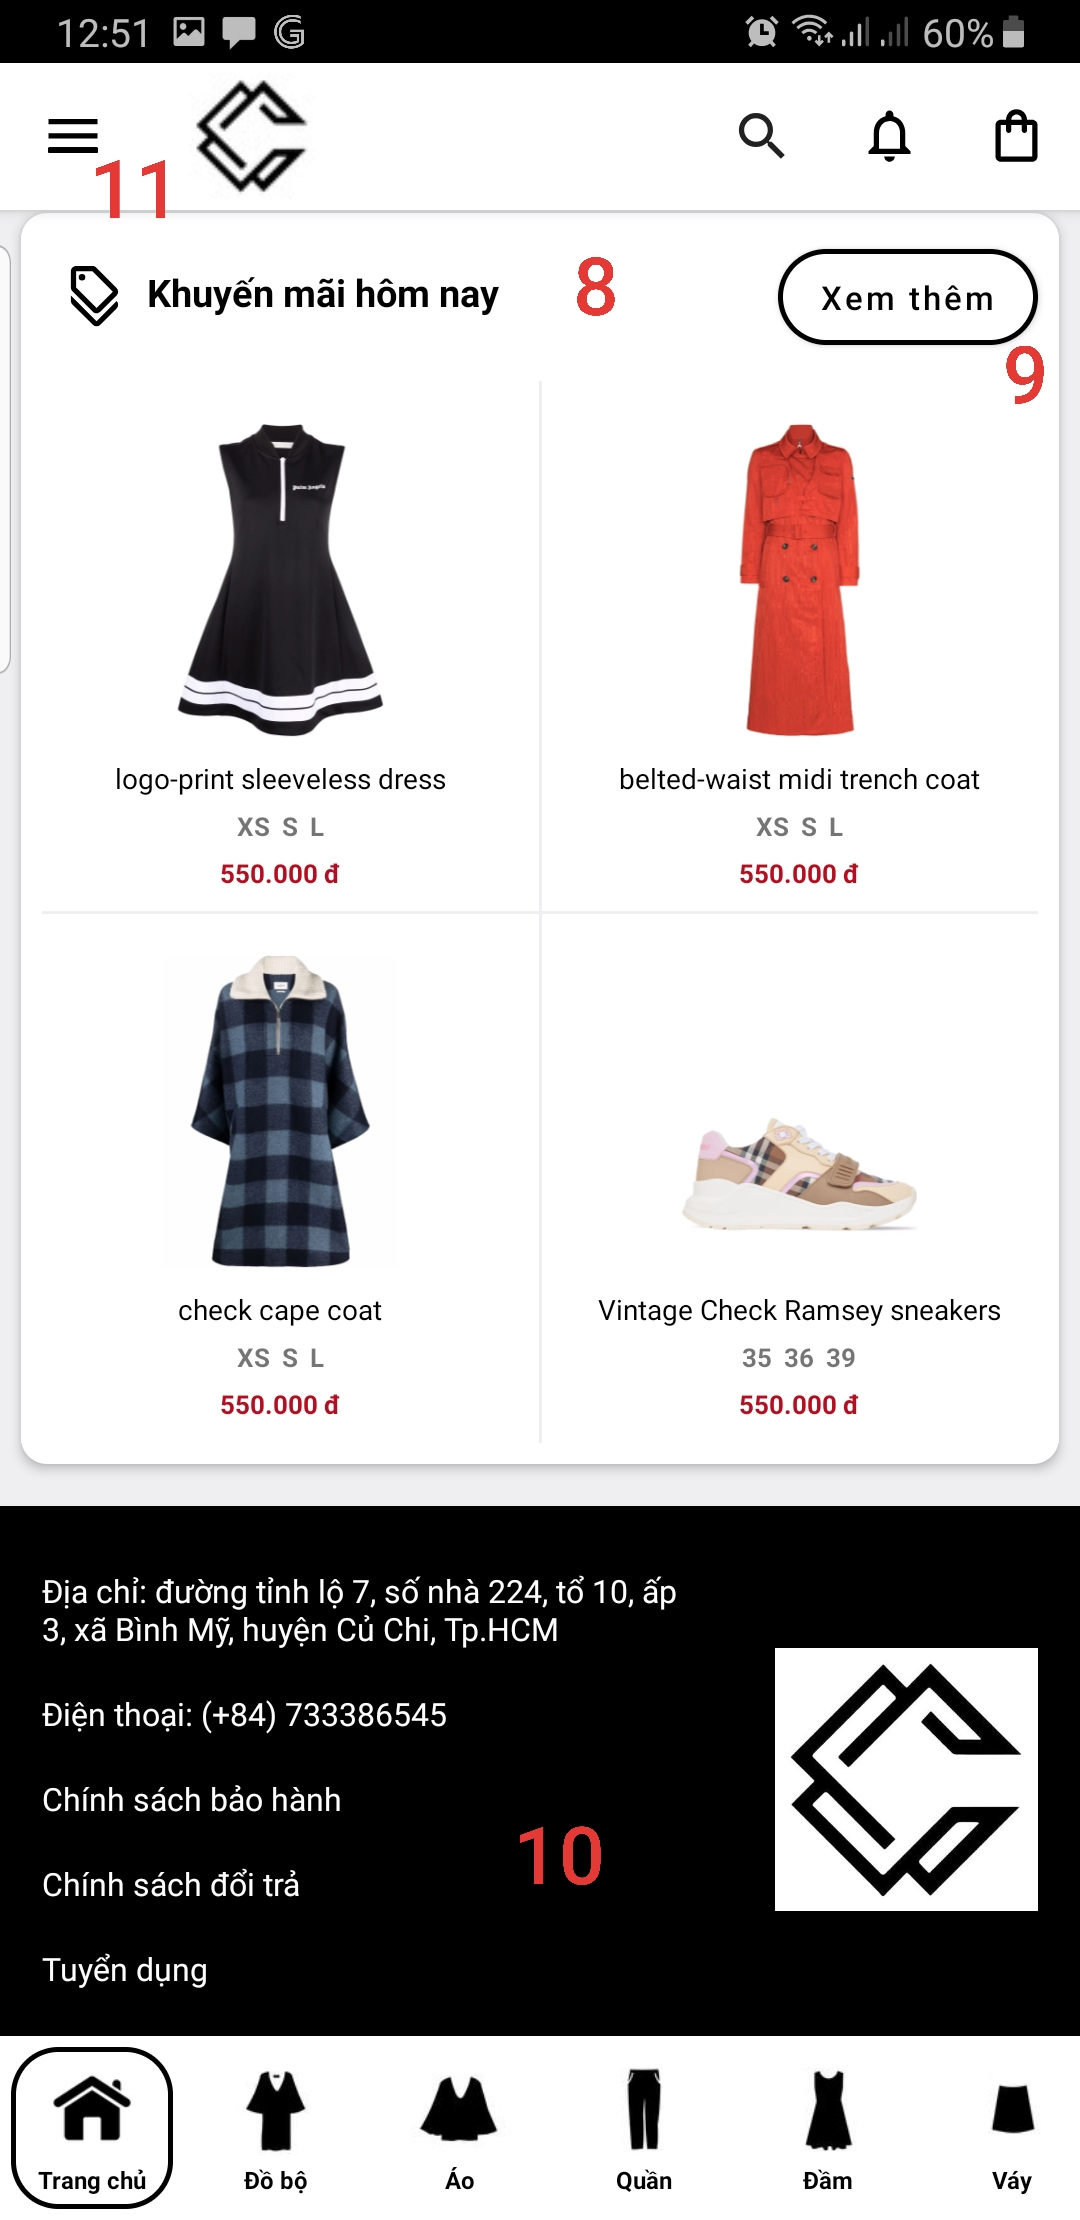
\includegraphics[height=10cm]{images/13.png}
    \caption{Màn hình trang chủ 3}
\end{figure}

\indent \textbf{Các thành phần và chức năng kèm theo trên màn hình (3)}
\begin{itemize}
    \item \textbf{8}: GridView - hiển thị bốn sản phẩm được khuyến mãi hôm nay. Nhấn vào item sẽ đứa đến trang chi tiết sản phẩm tương ứng, fragment này sẽ trình bày trong mục 2.3.4.
    \item \textbf{9}: Button - nhấn vào sẽ đưa đến một fragment khác hiển thị nhiều sản phẩm khuyến mãi hơn dưới dạng GridView, fragment này sẽ được trình bày ở mục 2.3.2.
    \item \textbf{10}: Footer - thể hiện địa chỉ, số điện thoại, các chính sách đổi trả, bảo hành của nhãn hàng.
    \item \textbf{11}: Hamburger toggle - nhấn vào để mở navigation view.
\end{itemize}

\newpage
\begin{figure}[H]
    \centering
    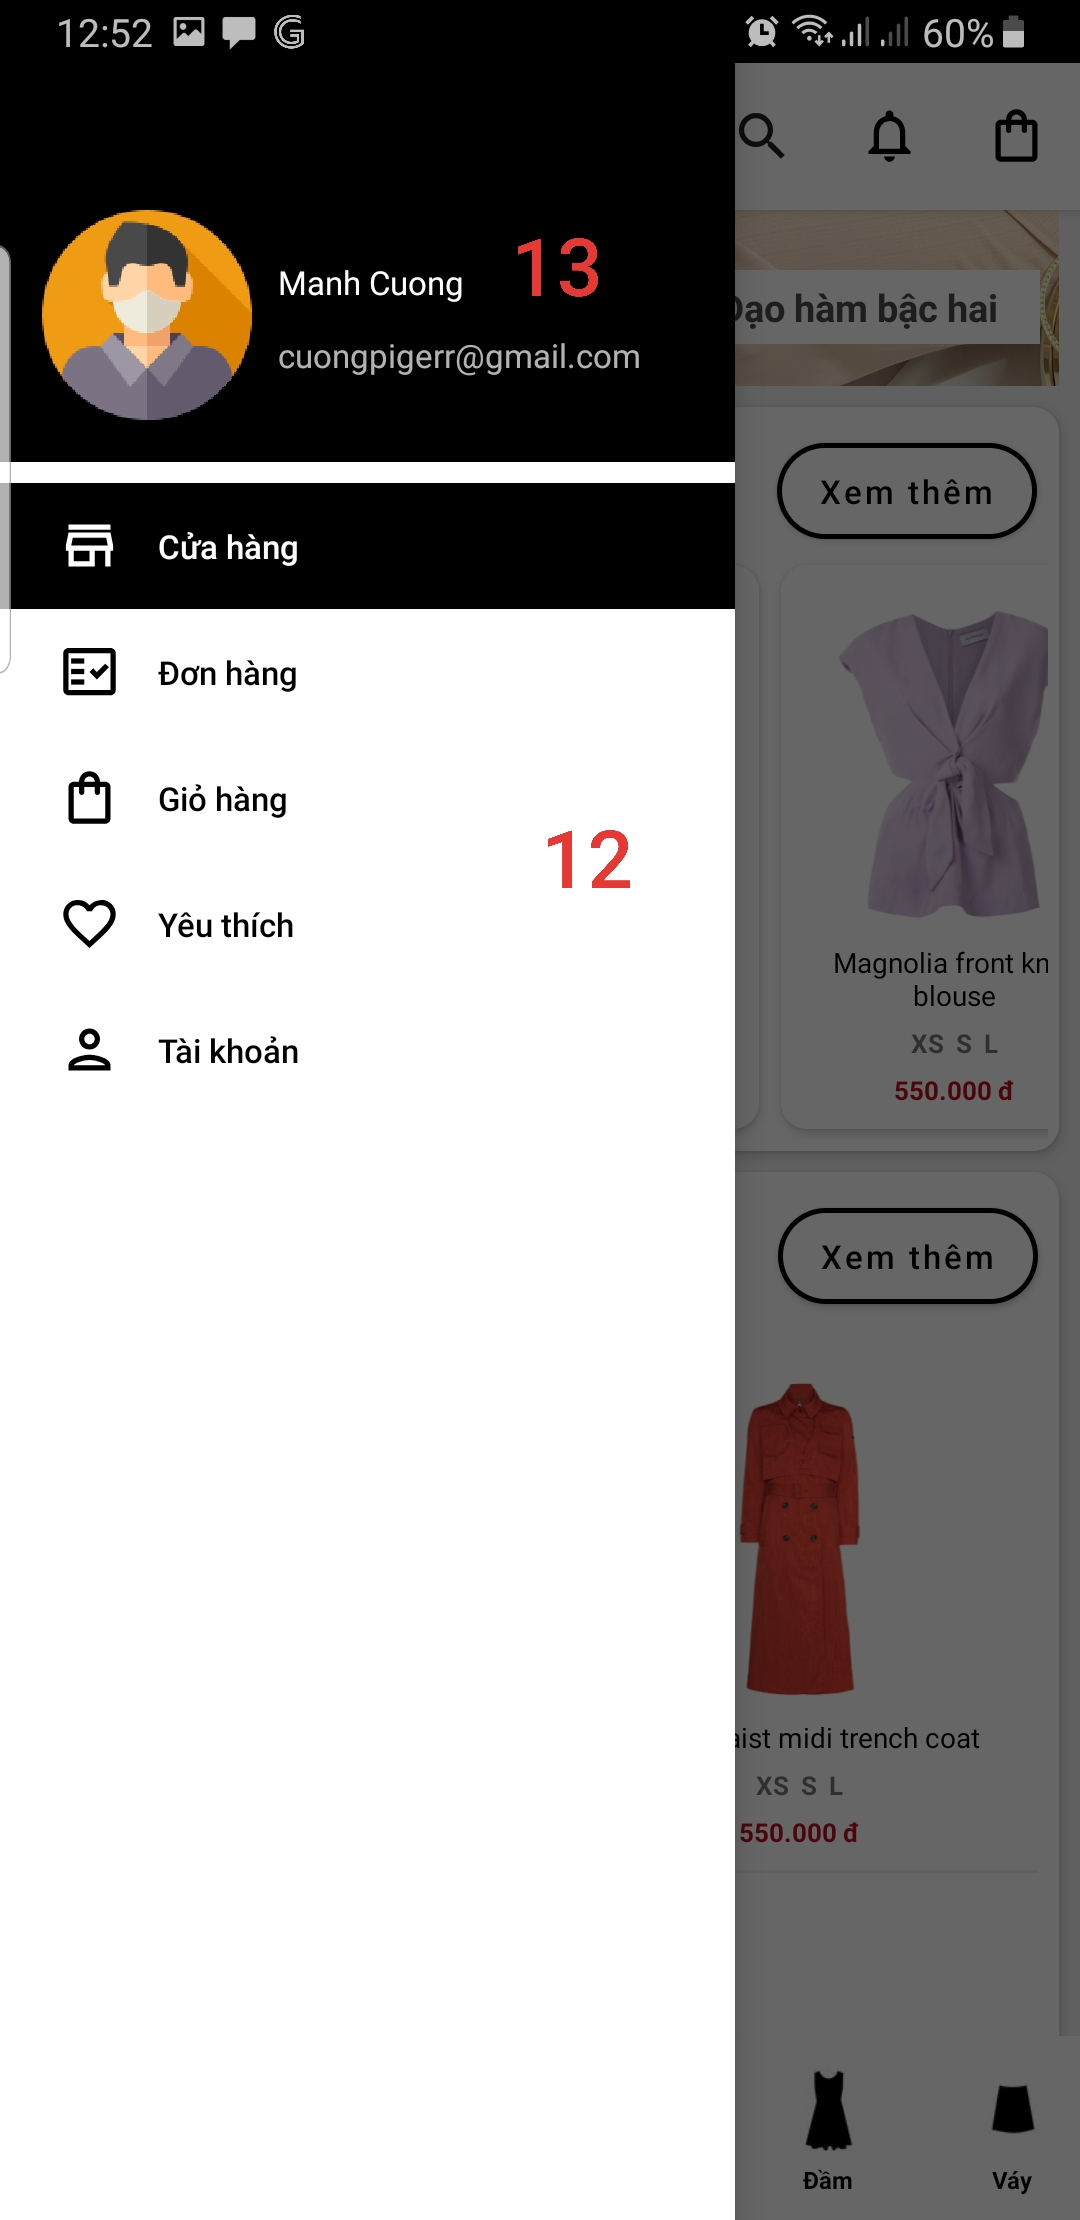
\includegraphics[height=10cm]{images/14.png}
    \caption{Màn hình trang chủ 4}
\end{figure}

\indent \textbf{Các thành phần và chức năng kèm theo trên màn hình (4)}
\begin{itemize}
    \item \textbf{12}: Navigation view - hiển thị các tab để đi đến các fragment khác của ứng dụng. Hiện tại ứng dụng đang ở fragment cửa hàng.
    \item \textbf{13}: Hai Textview - hiển thị tên người dùng và email nếu người dùng đã đăng nhập - ngược lại thì sẽ hiển thị thông báo chưa đăng nhập.
\end{itemize}

\indent \textbf{Ưu điểm}
\begin{itemize}
    \item Vì được thiết kế dưới dạng một Vertical Recycler View mà mỗi item là một container chứa tập các widget khác nhau, nên về sau ta dễ thêm bớt các container cho màn hình trang chủ.
\end{itemize}

\newpage
\subsubsection{Màn hình xem thêm sản phẩm}
Được thực hiện bởi sinh viên 20424008.\\

\indent Người dùng sẽ được đưa đến màn hình này khi nhấn vào thành phần \textbf{7} và \textbf{9} ở mục 2.3.1. Dưới đây là hình chụp màn hình này.

\begin{figure}[H]
    \centering
    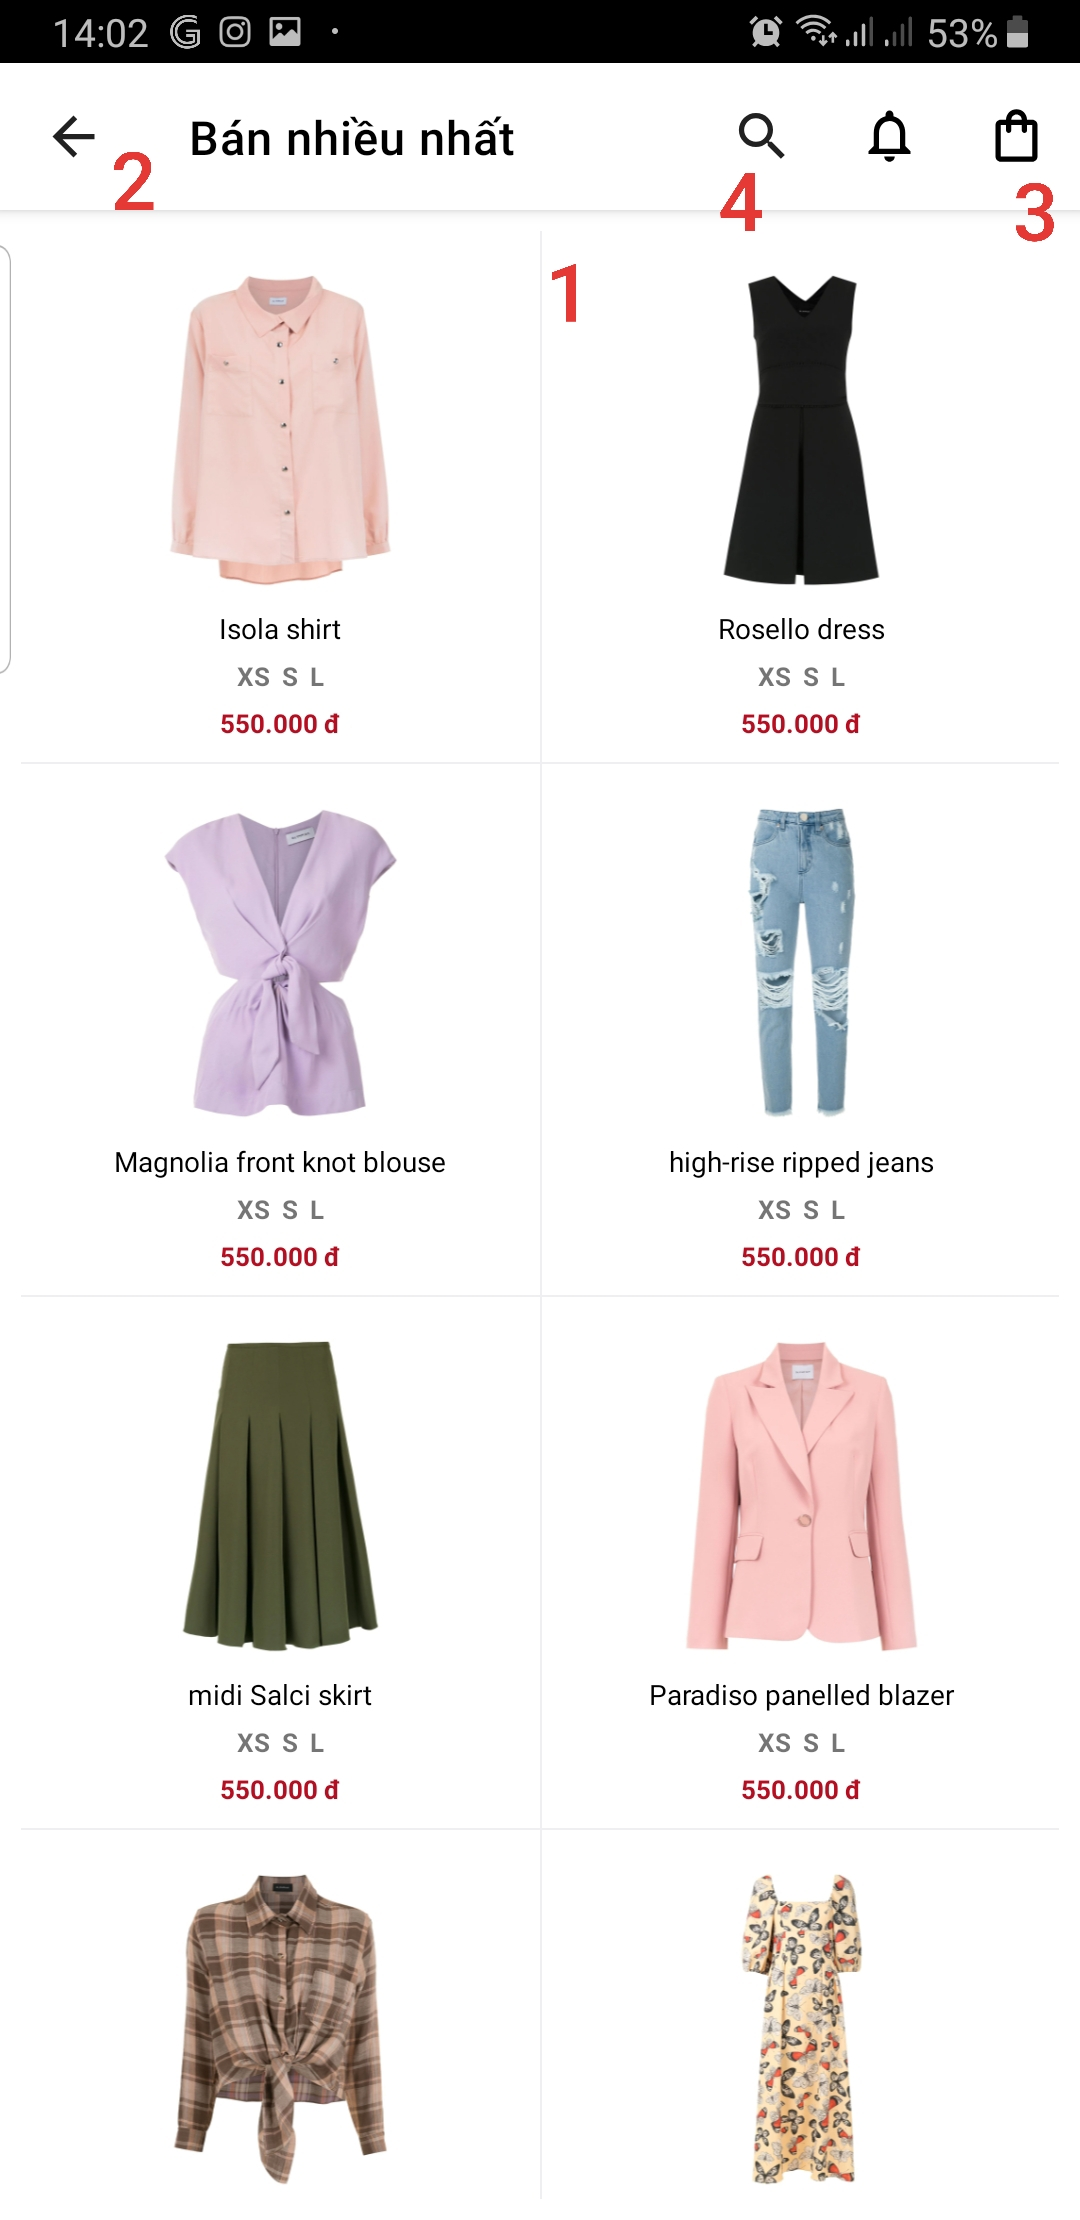
\includegraphics[height=10cm]{images/15.png}
    \caption{Màn hình xem thêm của các sản phẩm bán nhiều nhất (khi nhấn thành phần \textbf{7} ở mục 2.3.1)}
\end{figure}

\indent \textbf{Các thành phần và chức năng kèm theo trên màn hình (3)}
\begin{itemize}
    \item \textbf{1}: GridView - hiển thị nhiều hơn các sản phẩm khi người dùng nhấn vào thành phần \textbf{7} hoặc \textbf{9} ở mục 2.3.1. Có thể scroll, nhấn vào item để đi đến trang chi tiết sản phẩm tương ứng, fragment này sẽ trình bày trong mục 2.3.4.
    \item \textbf{2}: As home indicator - nhấn vào để quay về màn hình chính ở mục 2.3.1.
    \item \textbf{3}: Menu item Cart - nhấn vào để đến fragment giỏ hàng.
    \item \textbf{4}: Menu item Search - nhấn vào để thực hiện chức năng tìm kiếm.
\end{itemize}

\newpage
\indent Bên dưới là một vài hình ảnh thêm về màn hình này.

\begin{figure}[H]
    \centering
    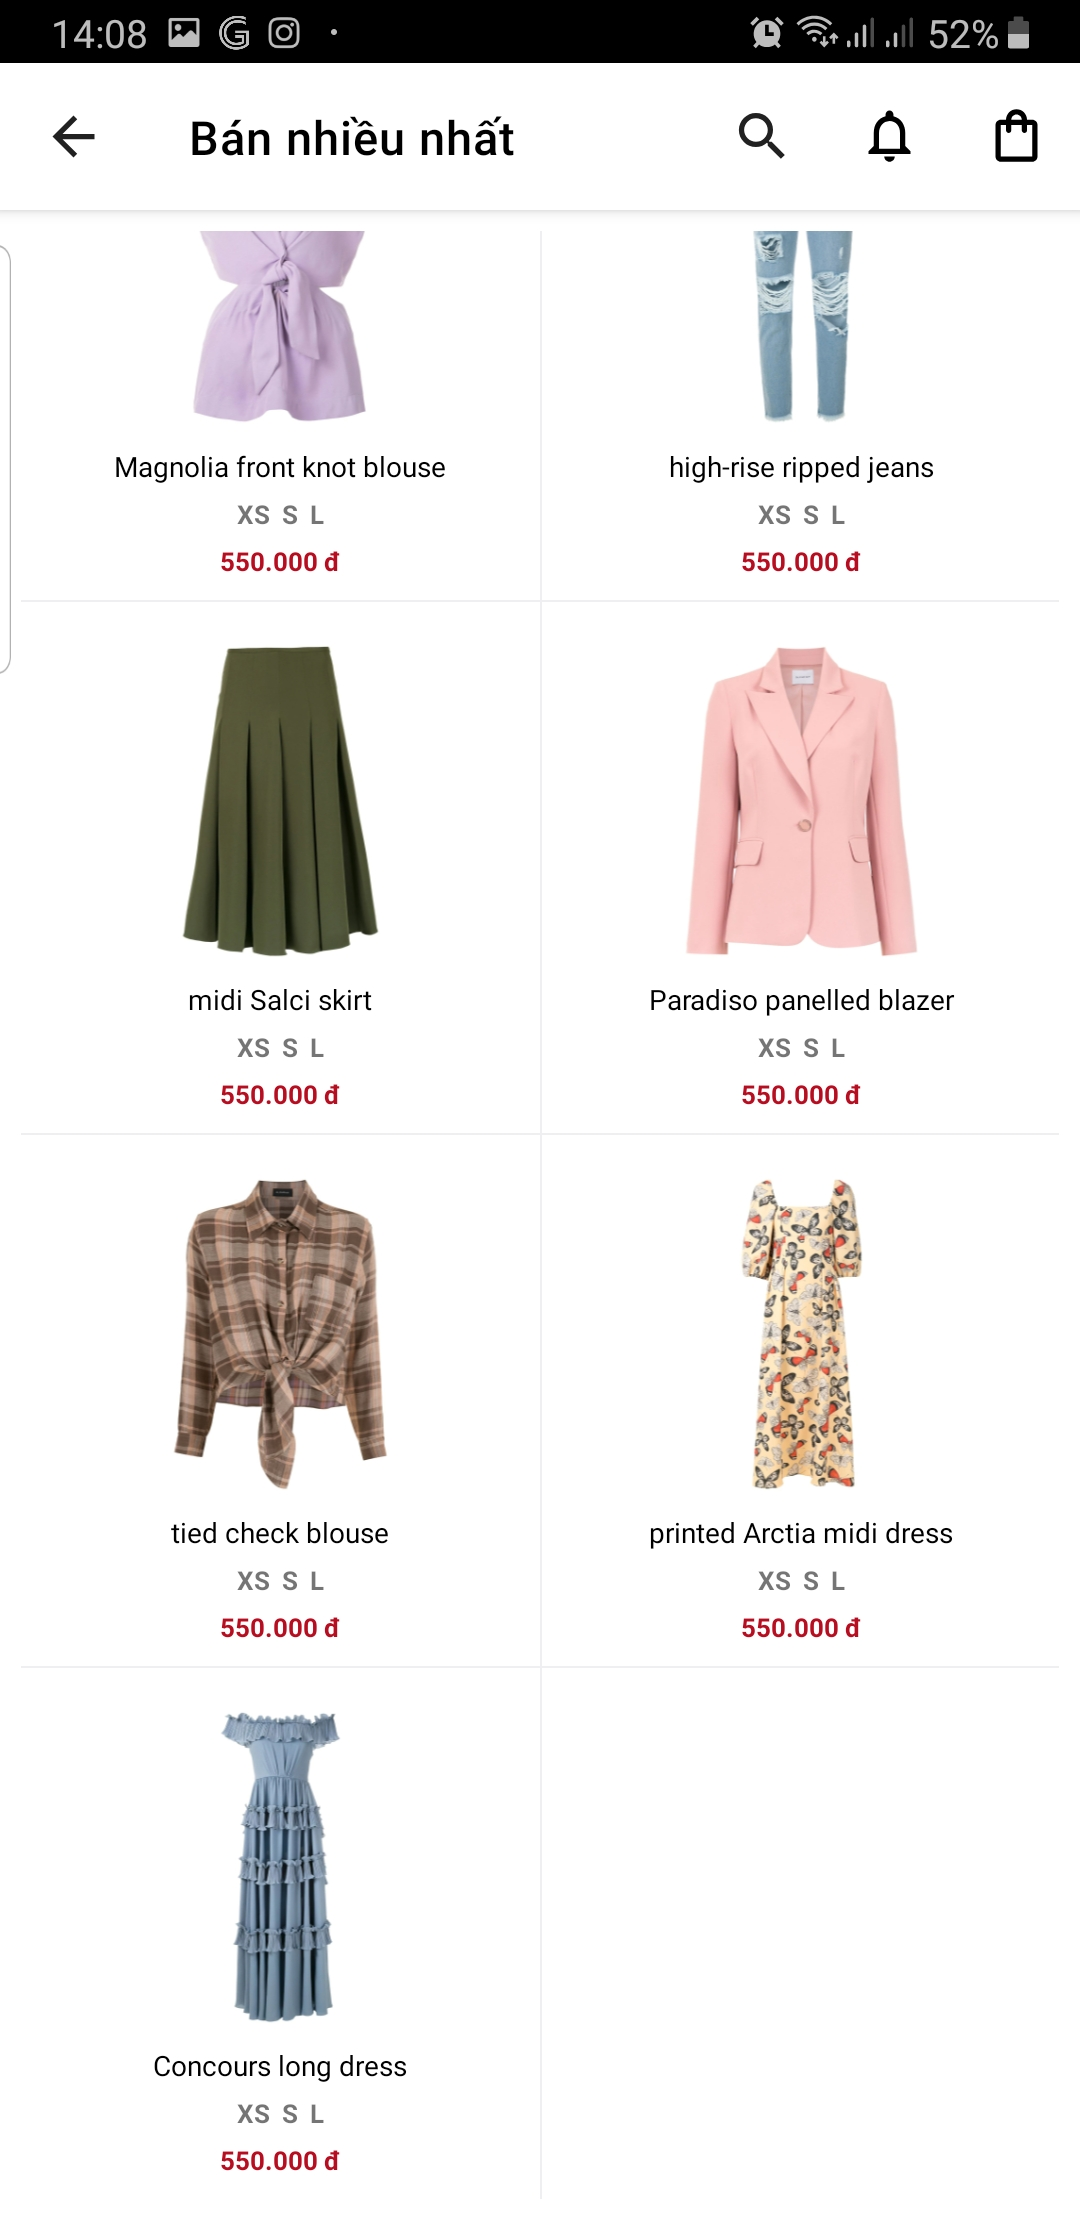
\includegraphics[height=10cm]{images/16.png}
    \caption{Màn hình xem thêm của các sản phẩm bán nhiều nhất - cuối trang (khi nhấn thành phần \textbf{7} ở mục 2.3.1)}
\end{figure}

\begin{figure}[H]
    \centering
    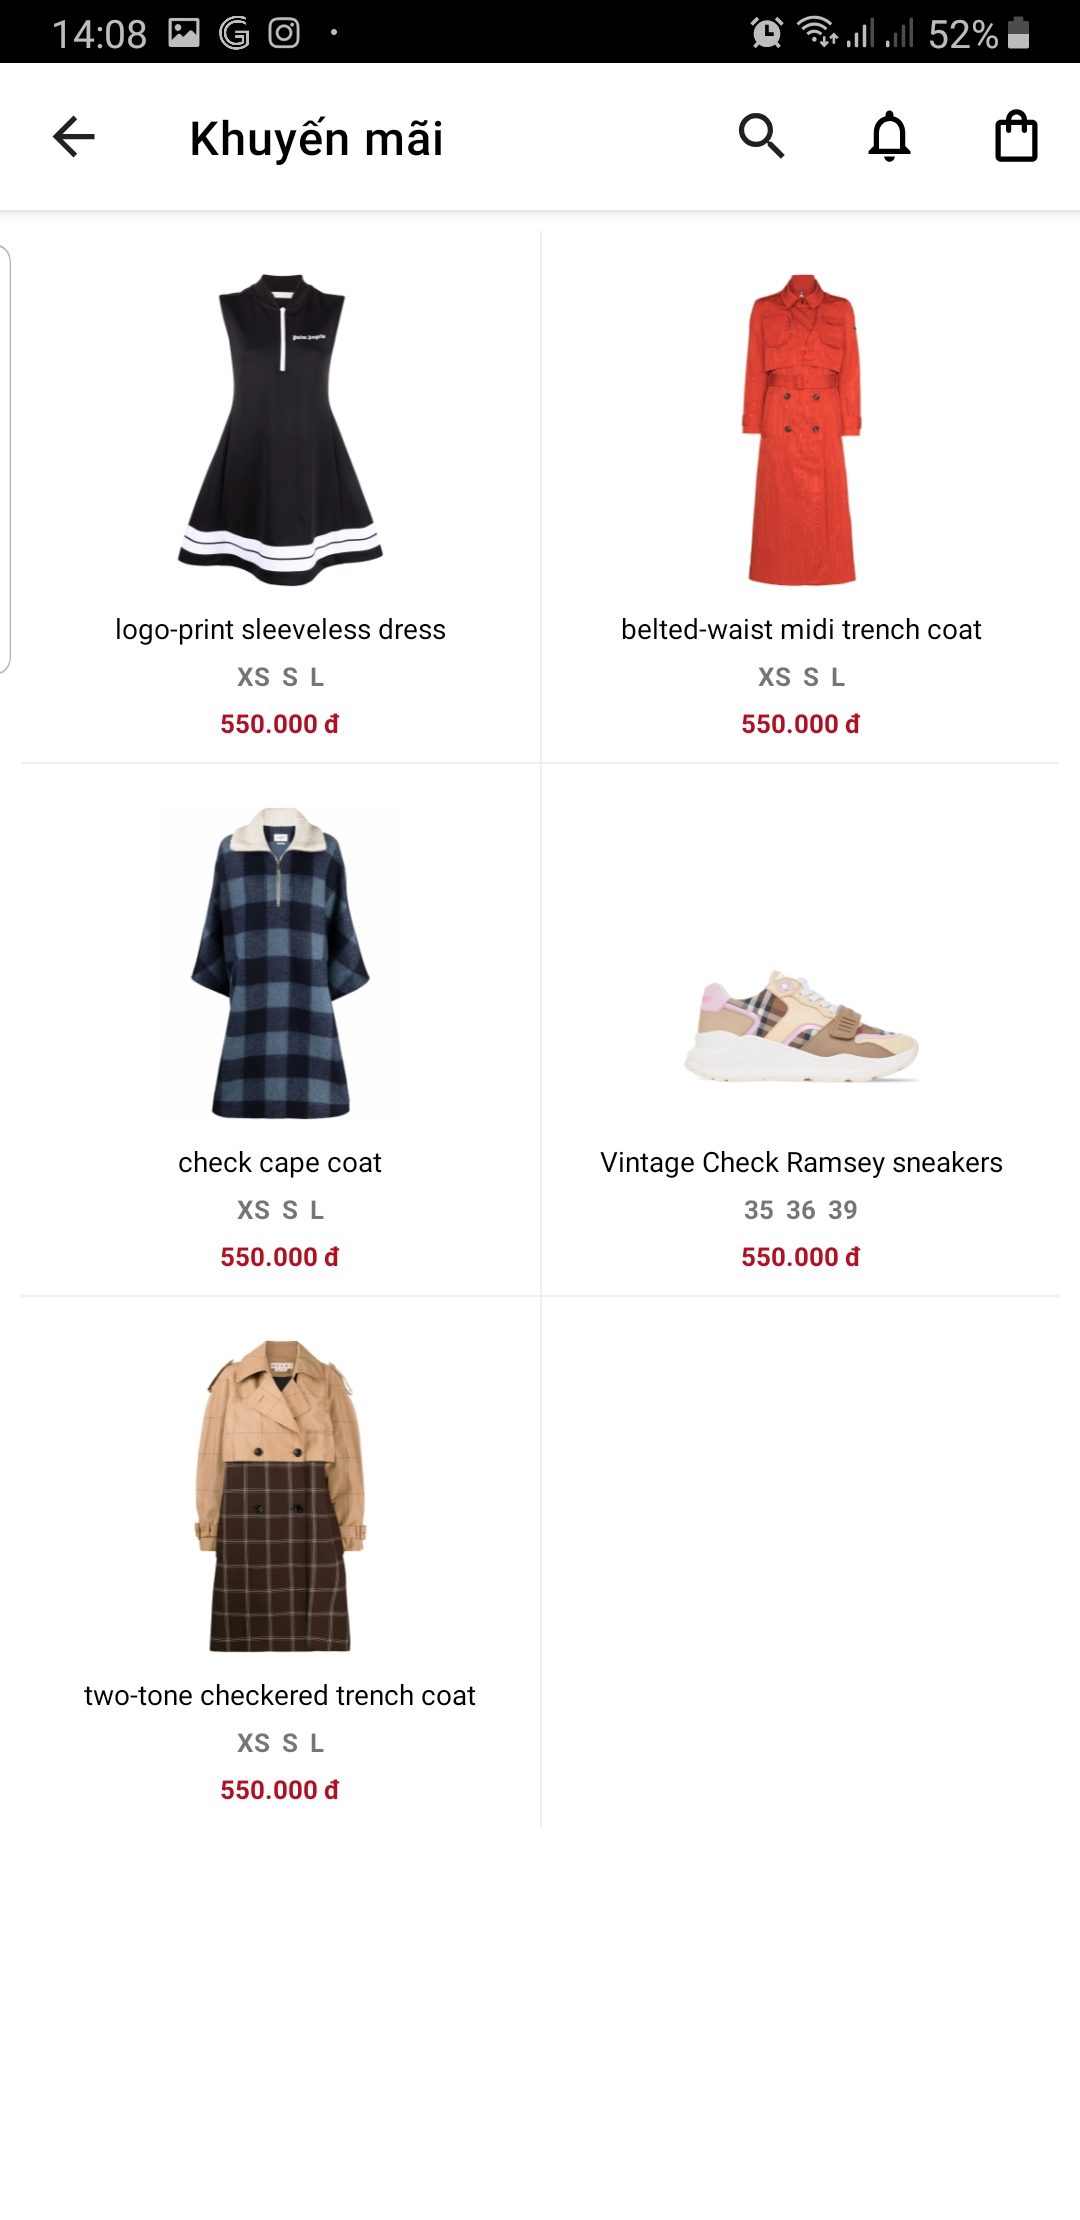
\includegraphics[height=10cm]{images/17.png}
    \caption{Màn hình xem thêm của các sản phẩm khuyến mãi (khi nhấn thành phần \textbf{9} ở mục 2.3.1)}
\end{figure}

\newpage
\subsubsection{Màn hình sản phẩm theo danh mục}
Được thực hiện bởi sinh viên 20424008.\\

\indent Màn hình này được chuyển đến khi người dùng nhấn vào các item trên thành phần \textbf{2} ở mục 2.3.1. Dưới đây là hình chụp màn hình này.

\begin{figure}[H]
    \centering
    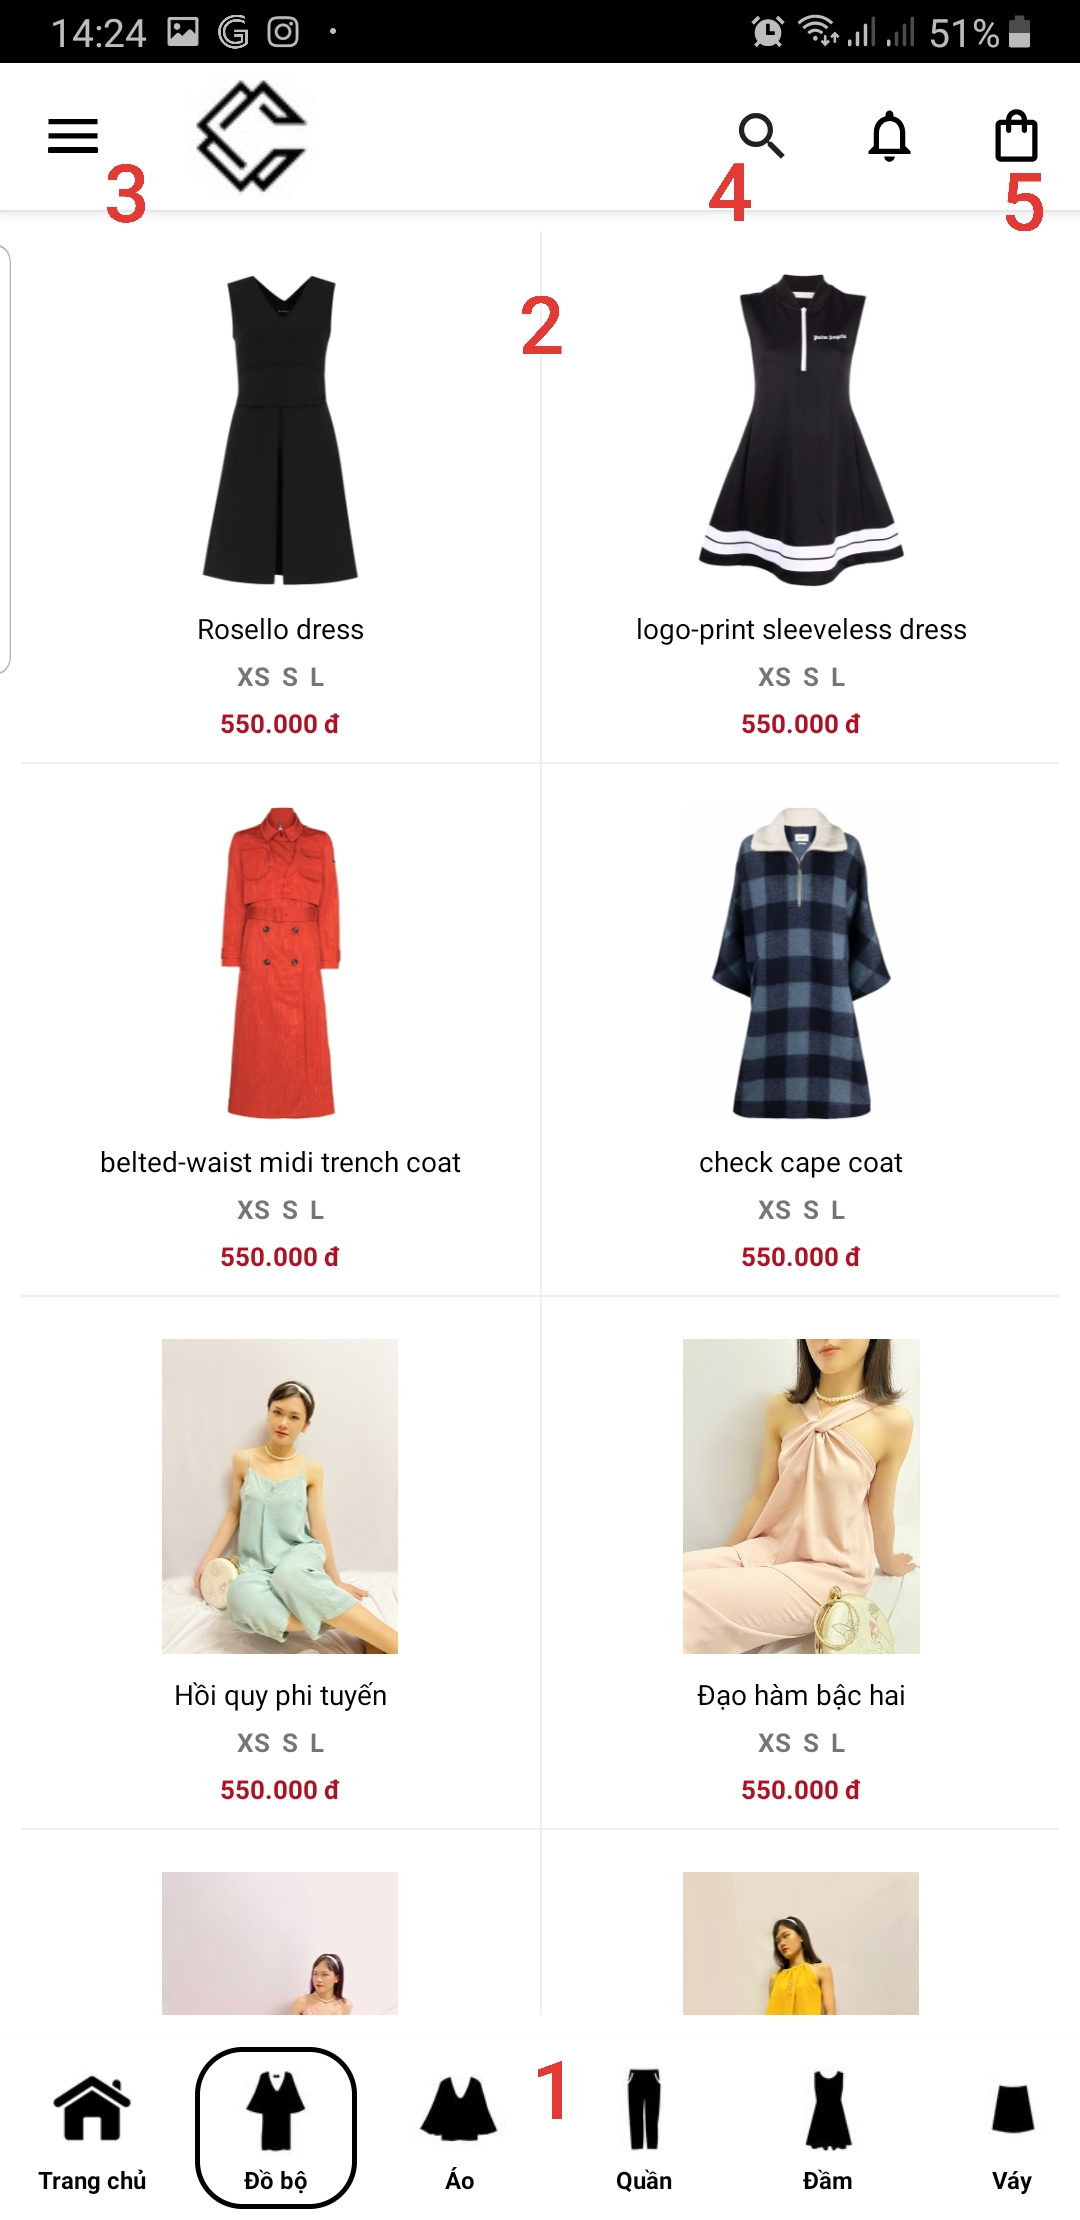
\includegraphics[height=10cm]{images/18.png}
    \caption{Màn hình xem các sản phẩm theo danh mục - danh mục "Đồ bộ"}
\end{figure}

\indent \textbf{Các thành phần và chức năng kèm theo trên màn hình}
\begin{itemize}
    \item \textbf{1}: Horizontal Recycler View - nhấn vào các item để đi đến các fragment của các danh mục sản phẩm khác
    \item \textbf{2}: GirdView - có thể scroll, nhấn vào các item để đi đến fragment chi tiết sản phẩm tương ứng, fragment này sẽ trình bày trong mục 2.3.4.
    \item \textbf{3}: Hamburger Toggle - nhấn để mở navigation view.
    \item \textbf{4}: Menu item Search - nhấn vào để thực hiện chức năng tìm kiếm.
    \item \textbf{5}: Menu item Cart - nhấn vào để đến fragment giỏ hàng.
\end{itemize}

\newpage
\indent Dưới đây là một vài hình ảnh thêm về màn hình này.
\begin{figure}[H]
    \centering
    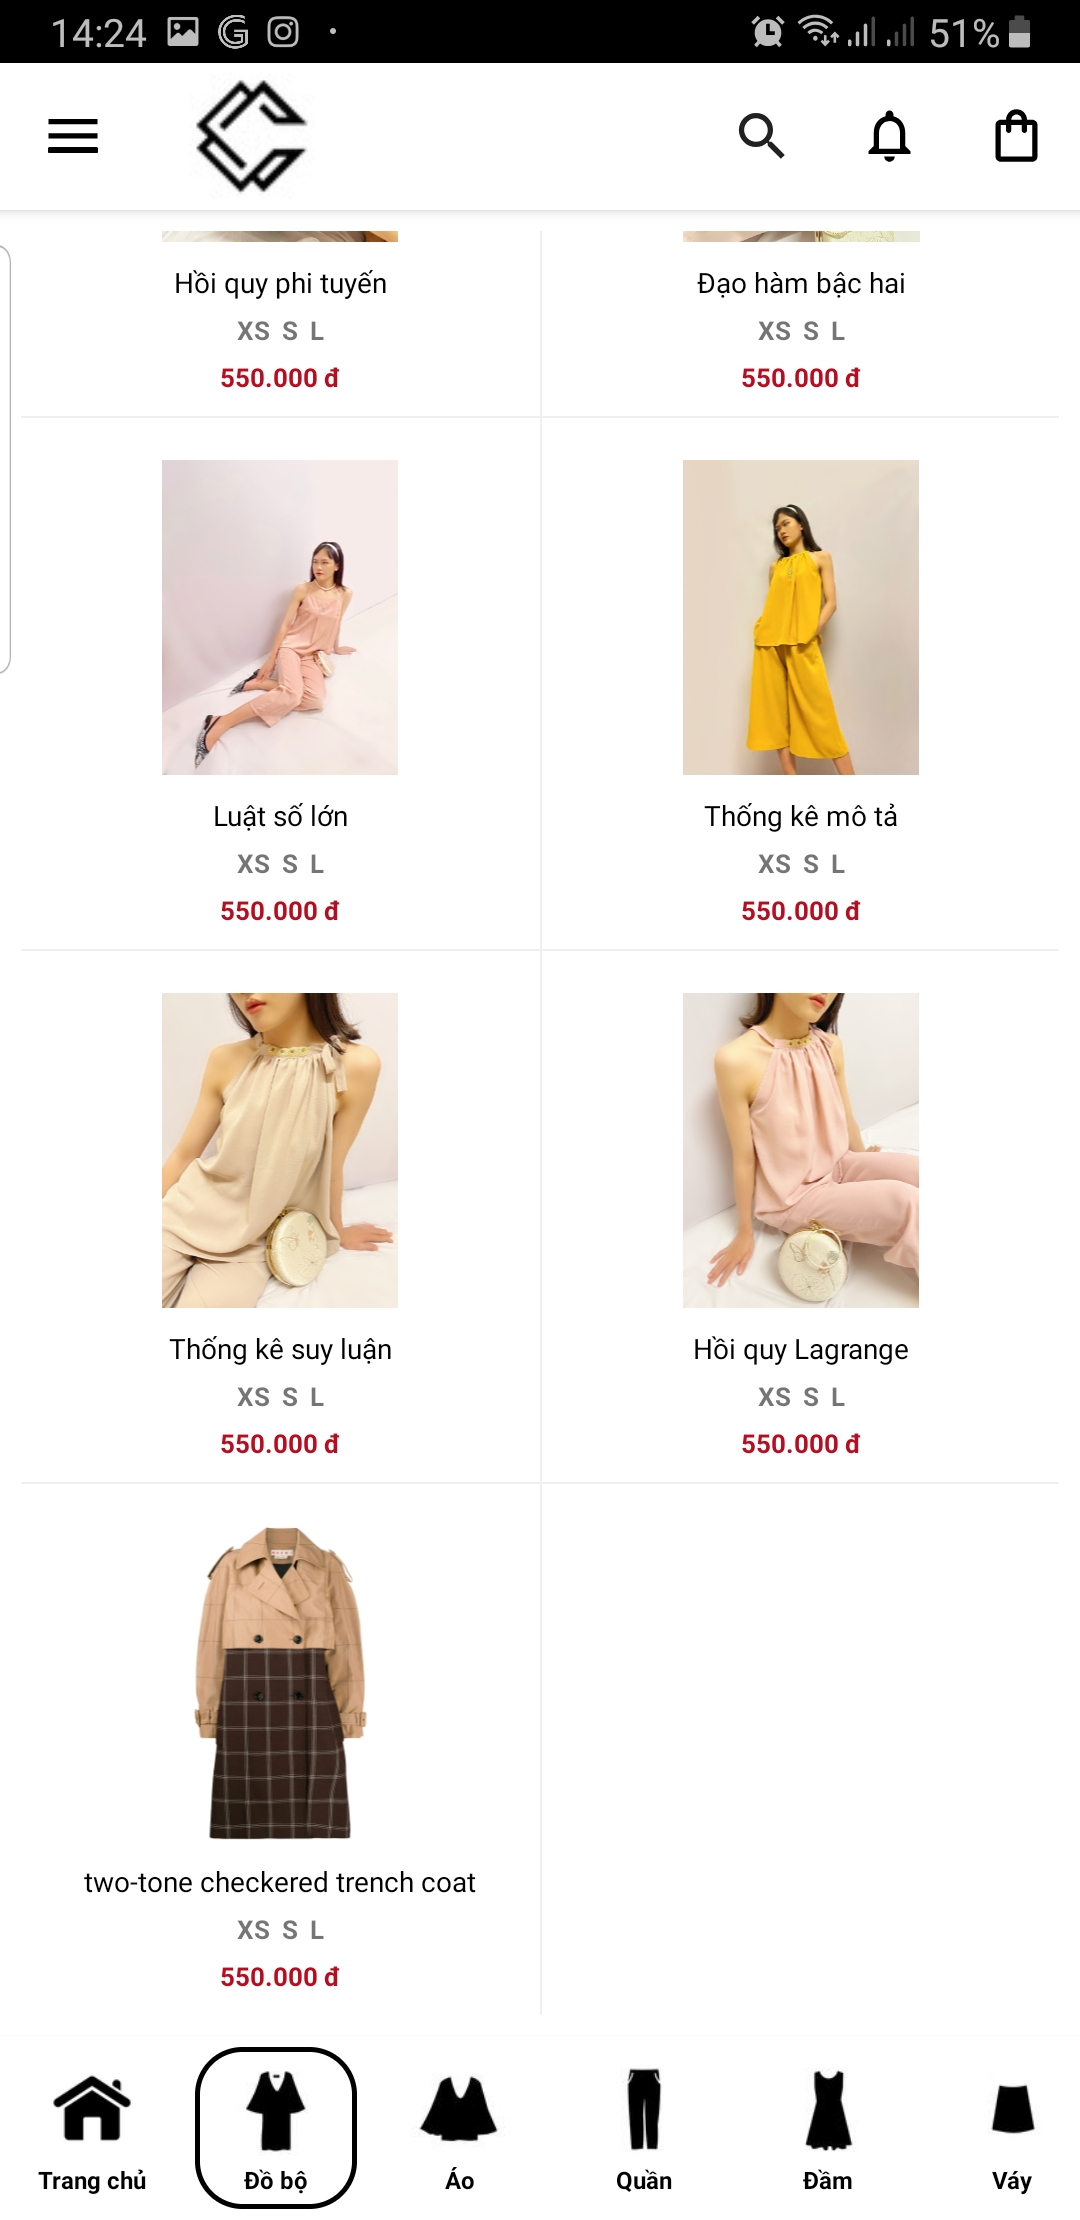
\includegraphics[height=10cm]{images/19.png}
    \caption{Màn hình xem các sản phẩm theo danh mục - cuối trang danh mục "Đồ bộ"}
\end{figure}

\begin{figure}[H]
    \centering
    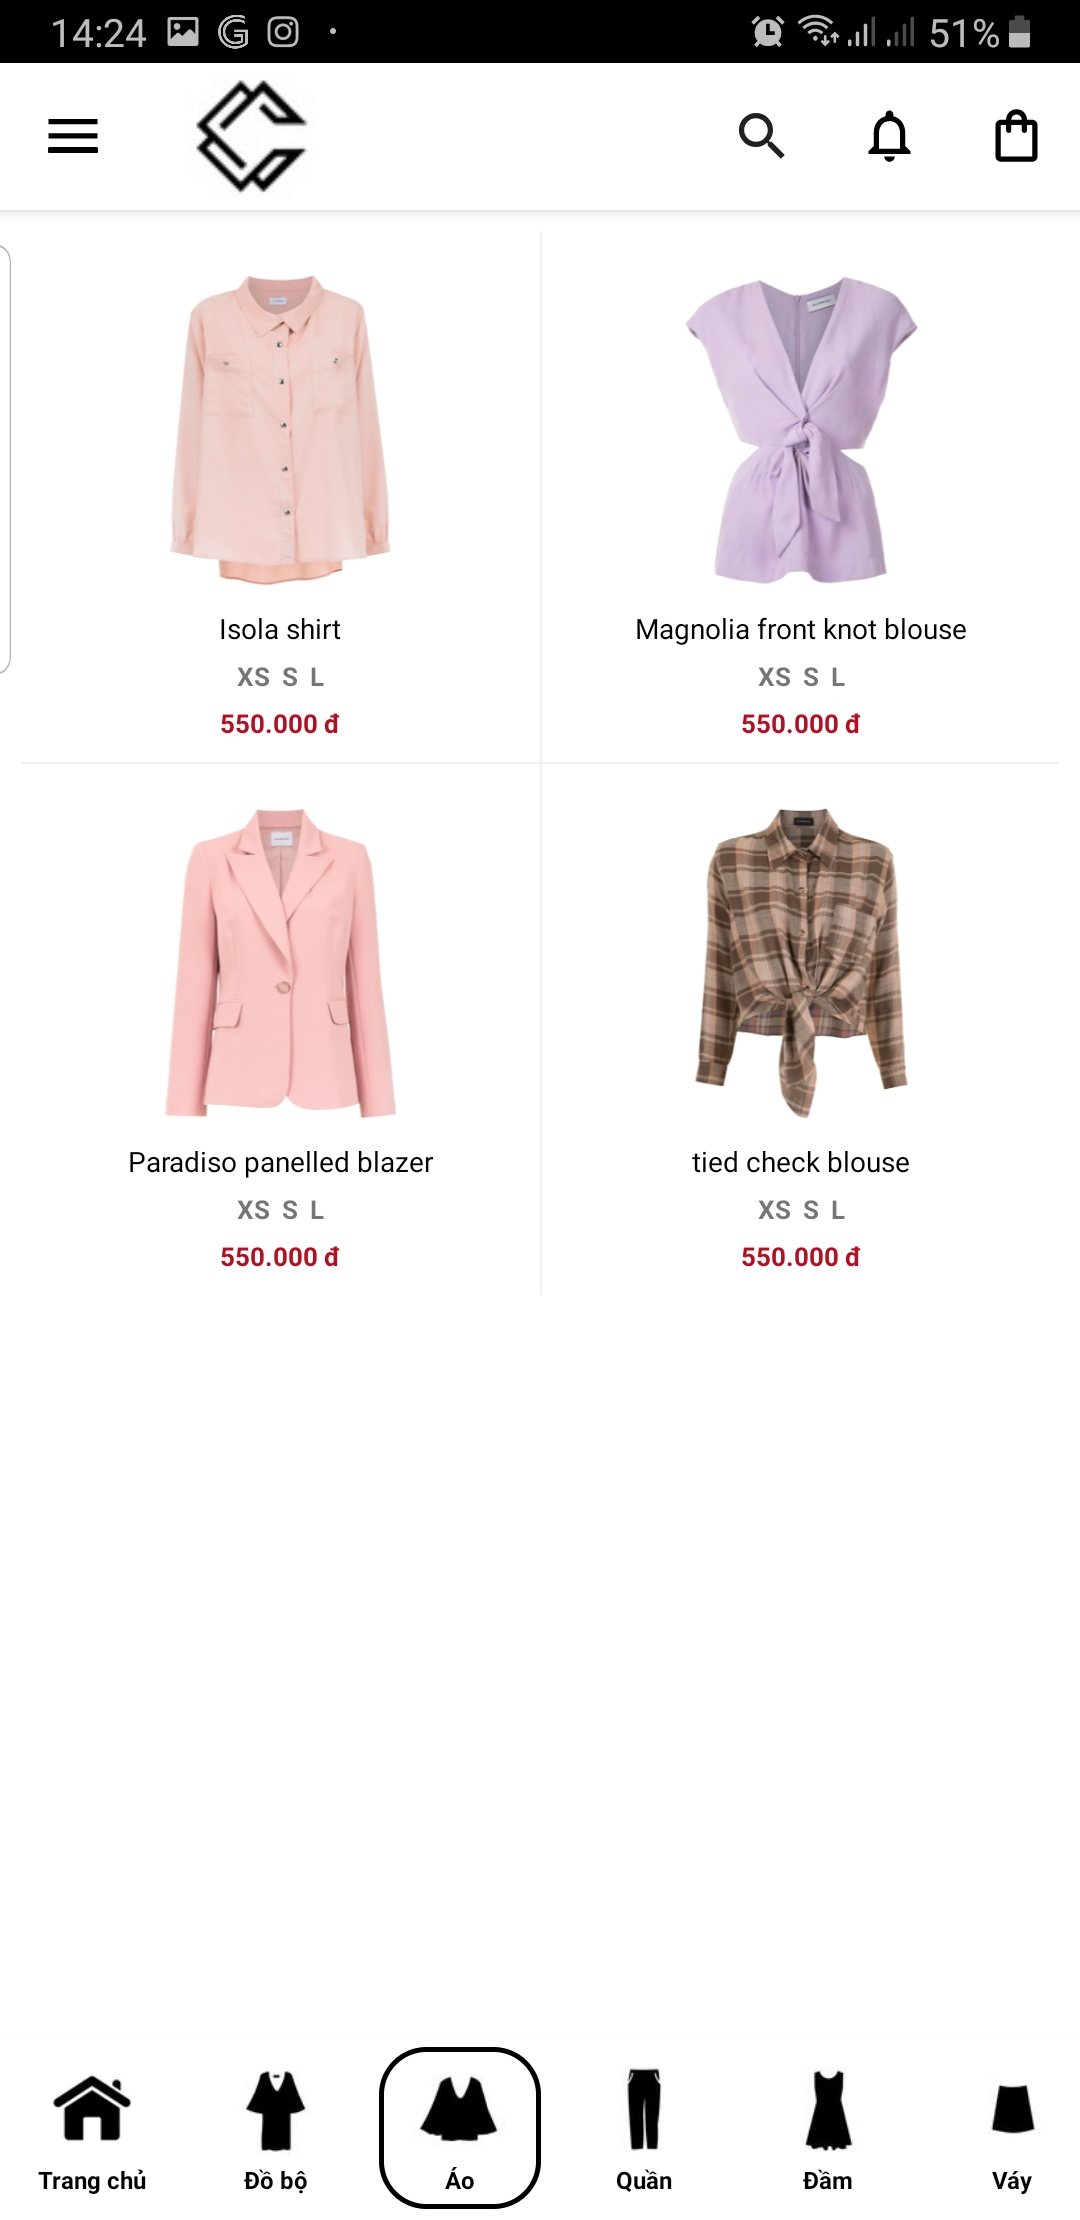
\includegraphics[height=10cm]{images/20.png}
    \caption{Màn hình xem các sản phẩm theo danh mục - danh mục "Áo"}
\end{figure}

\indent \textbf{Hạn chế}
\begin{itemize}
    \item Chưa có tính năng sắp xếp theo tiếu chí người dùng.
    \item Chưa có tính năng \textbf{Pull to load more} khi danh mục sản phẩm có nhiều sản phẩm, mặc định ứng dụng sẽ load toàn bộ sản phẩm tương ứng cho danh mục mà người dùng chọn.
\end{itemize}

\subsubsection{Màn hình chi tiết sản phẩm}
Được thực hiện bởi sinh viên 20424013.\\

\indent Màn hình này được chuyển đến khi người dùng nhấn vào các item của các thành phần \textbf{5, 6, 8} trong mục 2.3.1, thành phần \textbf{1} trong mục 2.3.2, thành phần \textbf{2} trong mục 2.3.3. Dưới đây là hình chụp màn hình này.

\end{document}